\section{Review reporting}

The selection process resulted in 20 papers, which were categorized using Wieringa's classification scheme \citep{wieringa2006requirements}. The following categories were relevant to this study:


\begin{itemize}
    \item Evaluation Research: Practical implementation and assessment of techniques or solutions, with a focus on investigating the outcomes.
    \item Validation Research: Examination of novel techniques in a controlled environment, typically a laboratory setting, before practical implementation.
    \item Solution Proposal: Presentation of a solution to a problem, highlighting its advantages, with a higher level of abstraction than validation research.
    \item Philosophical Paper: Introduction of a new perspective on existing concepts by structuring the field through a taxonomy or framework.
    \item Experience Paper: Narration of the author's personal experience, detailing what happened and how it occurred in practice.
    \item Opinion Paper: Expression of the author's personal viewpoint on a specific issue, without relying on related work or research methodologies.
\end{itemize}

The types of contributions were categorized as follows:
\begin{itemize}
    \item Model: Introduction of a new model or framework to address a specific problem.
    \item Method: Presentation of a new method or technique to solve a problem.
    \item Metric: Introduction of a new metric or evaluation criterion to assess the performance of a system or solution.
    \item Process: Description of a new process or workflow to improve efficiency or productivity.
    \item Tool: Introduction of a new tool or software application to facilitate a specific task or process.
\end{itemize}

Here is a systematic map of the selected papers, categorized by research type, contribution type and research question:

The table \ref{tab:systematicMap} presents a breakdown of research on various aspects of open-source software motivation, categorized by research methodology. The primary areas of interest are the factors motivating developers, the influence of social dynamics, and the obstacles to contribution. A significant majority of the studies (16 out of 20) employed evaluation research methods, primarily contributing models and methods to analyze these topics. While a few studies proposed solutions (3) or aimed to validate existing research (1), the emphasis on evaluation research indicates a strong focus on understanding and assessing the current landscape of open-source contributions.

\begin{table}[ht]
    \centering
    \begin{tabular}{| m{7em} | m{5.5em}| m{5.5em} | m{5.5em} | m{3em} |}
        \hline
                                 & Evaluation Research                                                  & Solution Proposal & Validation Research & Total \\
        \hline
        Motivation of developers & Model: P05, P09, P10, P13, P15, P16, P17, P18. Method: P08, P11, P12 & Process: P06      &                     & 12    \\ \hline
        Social dynamics impact   & Model: P20. Metric: P07                                              &                   & Metric: P19         & 3     \\ \hline
        Contribution barriers    & Model: P01, P04, P14                                                 & Model: P02, P03   &                     & 5     \\ \hline
        Total                    & 16                                                                   & 3                 & 1                   & 20    \\ \hline
    \end{tabular}
    \caption{Systematic map of selected papers}
    \label{tab:systematicMap}
\end{table}


\subsection{RQ1: Primary motivation for developers contributing in open source}

The primary aim of this research is to uncover the reasons why developers participate in OSS projects. Each study chosen for this analysis was examined for any empirically identified or assessed motivations, such as career advancement, skill development, altruism, or enjoyment. By understanding these motivations, I hope to gain insights into what drives individuals to contribute to OSS projects and how this knowledge can be used to foster greater participation and collaboration in the future.

A visual depiction of the quantity of published articles on the different incentives that encourage developers to contribute to open source software projects can be seen in the chart \ref{fig:articleMotivationCount}. The amount of articles devoted to each motivation is shown on the x-axis, while the motivations are grouped along the y-axis.

The data reveals a diverse range of motivations, with social factors emerging as prominent drivers of participation. The most extensively researched motivations, Signaling/Recognition (11 articles) and Play Value (10 articles), highlight the importance of social recognition and the inherent enjoyment developers derive from contributing to OSS projects. Personal Interest, Altruism and Ideology, and Learning also receive significant attention in the literature, with 8 articles dedicated to each. These motivations underscore the multifaceted nature of developer engagement, encompassing personal passions, a desire to contribute to the greater good, and the pursuit of knowledge and skill development.

Conversely, the least explored motivations are Role Transformation and Improving Software Quality, with only 2 articles each. This disparity suggests that while the existing literature acknowledges the potential impact of these motivations, they remain relatively understudied compared to social factors.

The diversity of motivations highlighted in the chart underscores the complexity of the open-source community. It is evident that developers are driven by a combination of social, personal, ideological, and career-oriented factors. This nuanced understanding is crucial for organizations and communities seeking to attract and retain developers. Tailored strategies that address the diverse motivations of developers are essential for fostering a thriving and sustainable open-source ecosystem.

Moreover, the chart reveals the need for further research into less-explored motivations, such as Role Transformation and Improving Software Quality. A deeper understanding of these motivations could provide valuable insights into how to incentivize contributions that directly enhance the quality and impact of OSS projects.

\begin{figure}[ht]
    \centering
    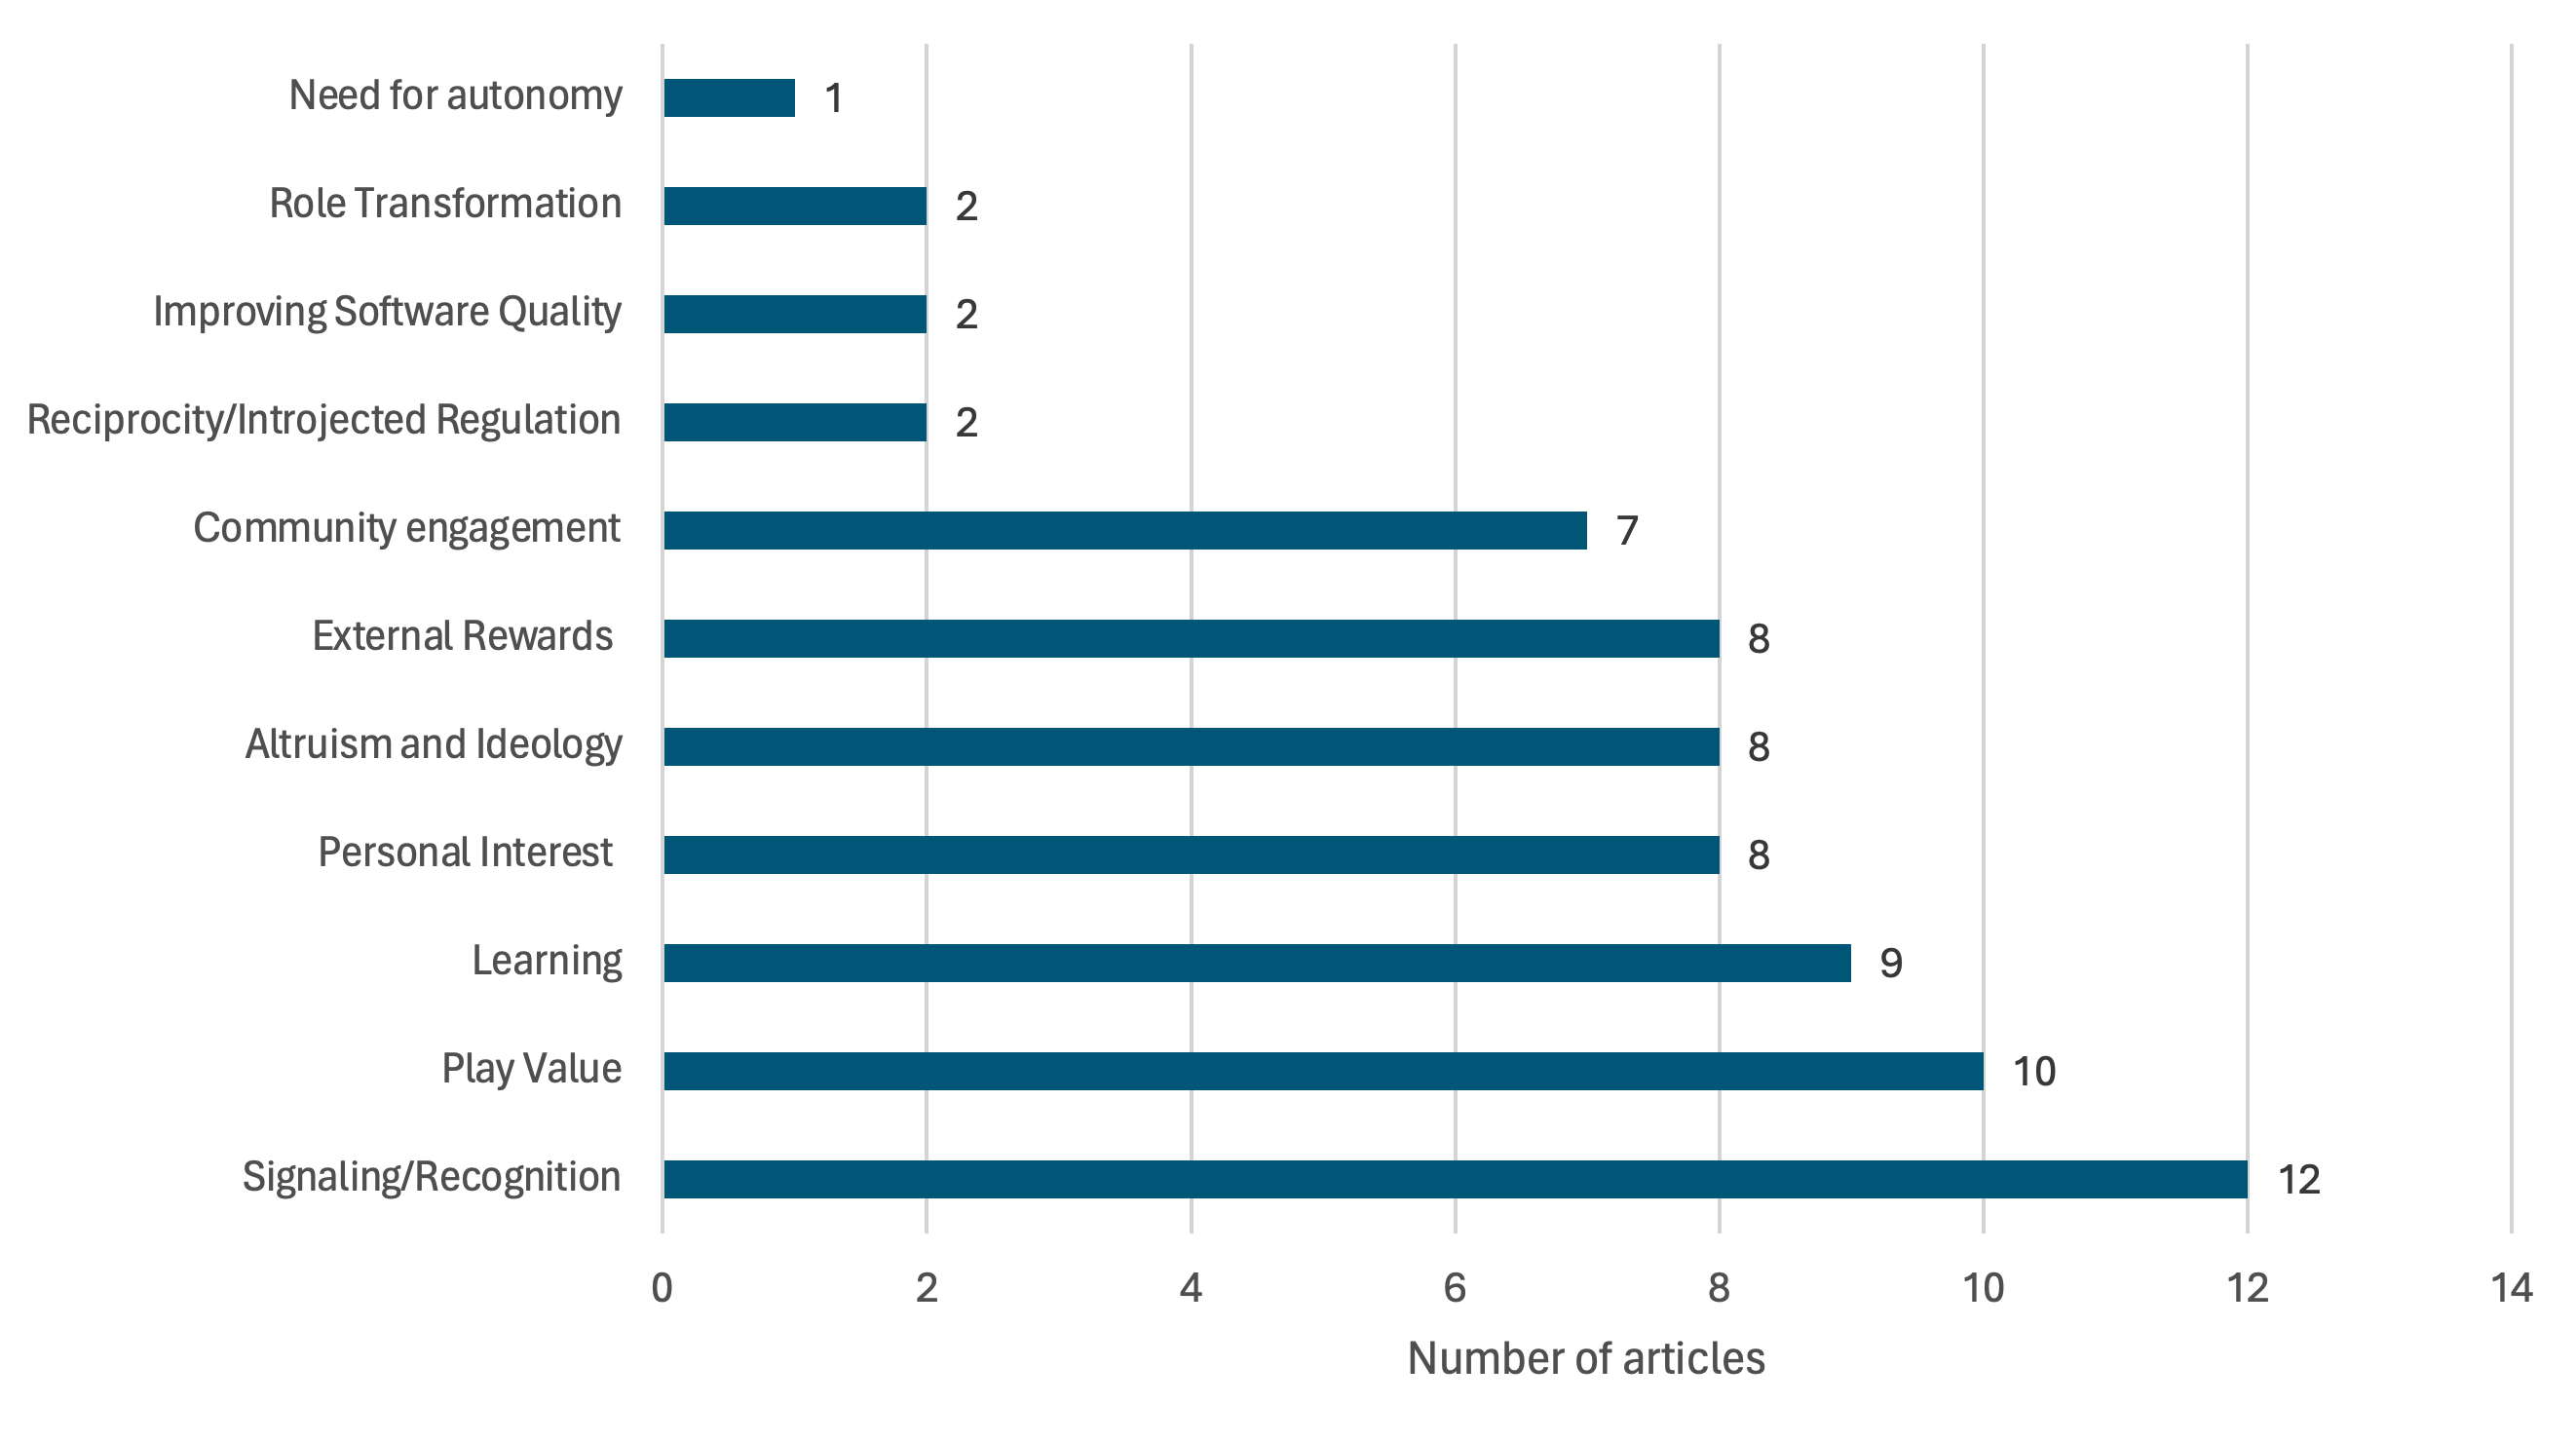
\includegraphics[width=1\linewidth]{figs/articleMotivationCount.png}
    \caption{Number of articles mentioning each motivation}
    \label{fig:articleMotivationCount}
\end{figure}

\subsubsection{Intrinsic motivations}
My exploration of developer motivation in open-source software projects begins with intrinsic motivations, the internal drivers that fuel participation for personal satisfaction rather than external rewards. This encompasses a broad spectrum of factors, including: play value, the inherent enjoyment derived from the coding process; community engagement, the sense of belonging and collaboration found within OSS projects; learning, the opportunity to develop new skills and expand technical knowledge; personal interest, the desire to work on projects that align with individual passions; altruism and ideology, the belief in contributing to a greater good and supporting the open-source philosophy; need for autonomy, the freedom to work independently and creatively; and reciprocity/introjected regulation, the desire to contribute back to the community and maintain a sense of personal responsibility for the project's success. I will delve deeper into each of these intrinsic motivations in the following sections, examining their unique influence on developer behavior within the OSS landscape.

1. Play value

In contrast to traditional software development, which often prioritizes external rewards like monetary compensation and career advancement, OSS projects offer a unique space where play value emerges as a central driving force. Play value, in this context, encapsulates the inherent enjoyment, intellectual stimulation, and creative fulfillment developers experience through the act of programming and problem-solving \parencite{05bitzer2007intrinsic, 06ye2003toward, 08zhang2024paid, 09lakhani2005hackers, 11gerosa2021shifting, 12choi2015characteristics,13li2012leadership,16ke2008motivations,17alexander2002working, 18oreg2008exploring}. Let's examine why this is such a powerful motivator.

For many developers, OSS represents a playground for experimentation and innovation. Unburdened by strict commercial deadlines or rigid specifications, they are free to explore novel ideas, test unconventional approaches, and engage in the iterative process of building software purely for the intrinsic satisfaction it provides .  The act of turning concepts into functional code can be deeply rewarding.

OSS communities often tackle complex technical problems that demand creative solutions.  Developers who are drawn to intrinsically motivating challenges revel in the opportunity to dissect intricate issues, devise elegant workarounds, and optimize code performance. This continuous learning process creates a sense of mastery and accomplishment that fuels further engagement.

Commercial software development typically necessitates compromises – feature trade-offs, adherence to proprietary standards, and prioritization of market demands over pure technical curiosity. In contrast, OSS projects offer developers a liberating space to exercise their technical creativity without external pressures. This autonomy nourishes problem-solving and innovation for its own sake.

The collaborative aspect of OSS can itself be a form of play.  Engaging with fellow developers, brainstorming solutions, exchanging knowledge, and contributing to a shared creation can be intellectually stimulating and enjoyable. This connection fosters a playful sense of experimentation and discovery within the community.


2. Community engagement

The act of conceptualizing the open-source community as a metaphorical family, united in pursuit of shared objectives, can be a powerful catalyst for developer participation \parencite{05bitzer2007intrinsic,07zhao2024openrank, 08zhang2024paid, 09lakhani2005hackers, 13li2012leadership, 16ke2008motivations, 17alexander2002working}. This collaborative environment fosters contributions aimed at communal advancement, even when they may not yield immediate personal gain for the individual developer. Participation in open-source projects can be fueled by a profound sense of belonging and an alignment of personal values with those of project teams and the open-source movement at large.

The chart \ref{fig:motivationDimension} underscores the complex interplay of motivations that drive developer participation in open-source projects. While social factors are paramount, career considerations and political beliefs also play a significant role. This diversity of motivations highlights the need for a nuanced understanding of the open-source community and tailored strategies to attract and retain developers.

\begin{figure}[ht]
    \centering
    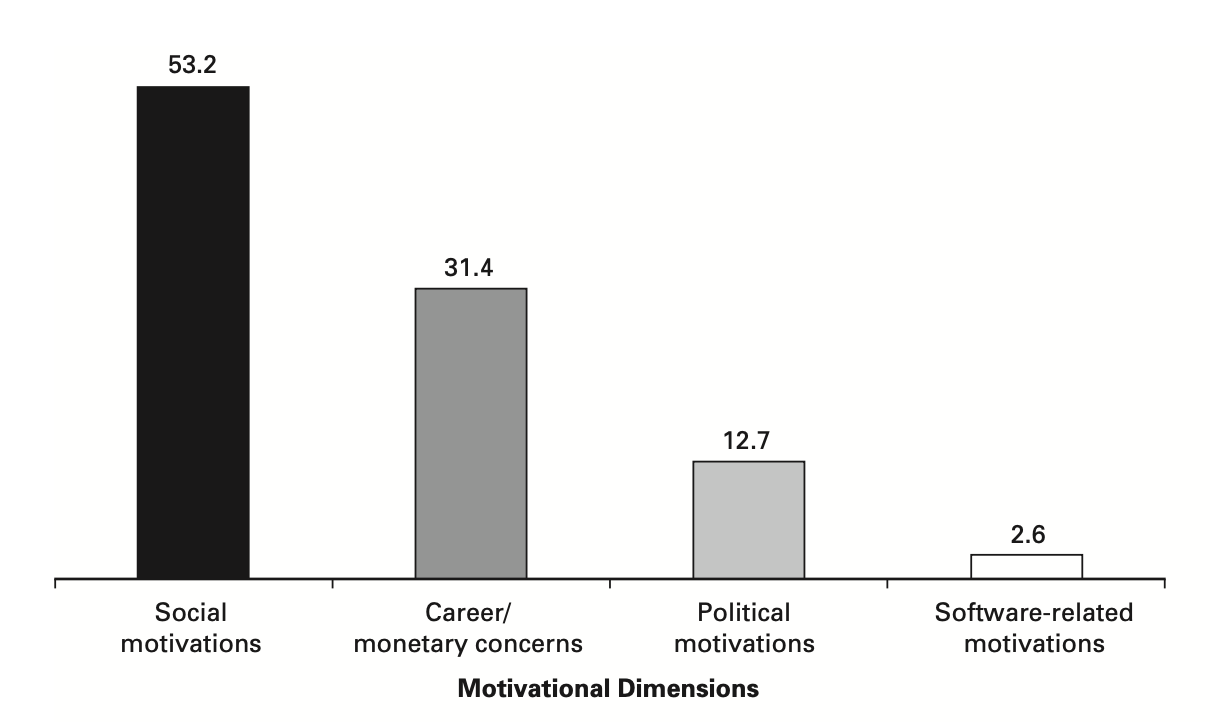
\includegraphics[width=0.7\linewidth]{figs/motivationDimension.png}
    \caption{As a proportion of all contributors to OSS, developers by motivation class \citep{ghosh2002free}}
    \label{fig:motivationDimension}
\end{figure}

Additionally,  a conviction regarding the inherent value of open-source code, paired with a perceived responsibility to contribute to the free and OSS ecosystem, serves as a significant motivator for developers. Cultivating a sense of belonging and fostering a shared purpose within the community or project team can thus be instrumental in empowering individuals to become active participants and contributors in the open-source software development landscape.



3. Learning

Research consistently identifies learning as a primary impetus for individuals to actively engage in OSS communities \parencite{06ye2003toward, 07zhao2024openrank, 08zhang2024paid, 09lakhani2005hackers, 10wu2007empirical, 11gerosa2021shifting, 12choi2015characteristics, 17alexander2002working, 18oreg2008exploring}. OSS projects present multifaceted learning environments; developers are drawn to the inherent opportunities to acquire knowledge from the systems themselves, to collaborate and gain insights from fellow community members, and to reciprocally disseminate their own expertise.

Participation within OSS communities extends beyond the purely technical exchange of knowledge, encompassing a rich social dimension. By directly engaging in open-source projects, developers immerse themselves in a collaborative network of peers, often spanning skill levels and expertise. This fosters a dynamic learning ecosystem where individuals benefit from informal mentorship opportunities, observing problem-solving approaches employed by more experienced contributors, and receiving constructive feedback that accelerates their professional growth.

Moreover, the act of contributing to a shared knowledge base empowers developers and reinforces self-efficacy. The potential for continuous self-development, the pursuit of mastery, and the ability to give back to a community dedicated to knowledge-sharing serve as profound and enduring sources of motivation for many software contributors.

4. Personal interest

Some developers get involved in open-source projects due to a personal interest in the subject matter or a desire to address a specific need or problem. This intrinsic motivation is driven by a passion for the technology, a curiosity about the project's objectives, or a personal connection to the software's utility. Developers who are personally invested in the project's success are more likely to contribute actively and engage with the community \citep{06ye2003toward,07zhao2024openrank,09lakhani2005hackers,11gerosa2021shifting,12choi2015characteristics,13li2012leadership,16ke2008motivations,17alexander2002working}

The concept of the "personal itch," as articulated by Eric S. Raymond, illuminates a key motivator for developer participation in OSS projects \citep{holtgrewe2004articulating}. Individuals often engage in OSS development to address a specific problem or augment functionality that directly aligns with their personal or professional needs. The desire to create a solution that may not otherwise exist, driven by this personal necessity, serves as a potent catalyst for engagement.

Furthermore, the inherent intellectual challenge of solving complex programming problems stands as a significant motivator for developers seeking to contribute to open-source initiatives. The opportunity to grapple with intricate coding puzzles, apply problem-solving strategies, and ultimately contribute to the solution can be deeply fulfilling for those driven by a passion for programming.

The sense of creativity fostered within the OSS landscape is another powerful draw. Developers are empowered to express their ingenuity, explore innovative solutions, and continuously hone their skills through the development of tools or solutions that serve their own requirements or those related to their work. This blend of personal utility, creative expression, and continuous learning establishes a compelling environment that attracts and sustains developer involvement.

5. Altruism and ideology

OSS development thrives in part due to the contributions of individuals motivated by altruism and ideological convictions \citep{07zhao2024openrank,08zhang2024paid,10wu2007empirical,11gerosa2021shifting,13li2012leadership,16ke2008motivations,17alexander2002working,18oreg2008exploring}. This section explores these factors and their influence on developer participation. A significant driver for many developers is the inherent satisfaction derived from assisting others. Contributing to open-source projects allows them to directly improve software used by a wider community. This collaborative environment fosters a sense of purpose, as developers witness the positive impact of their work on others

Many developers are drawn to  the core principles of open-source software, including transparency, collaboration, and the democratization of technology. Participation allows them to contribute to a development model that emphasizes open access and fosters a sense of community.  Additionally, developers can be motivated by a desire to create software that benefits the greater good by being freely available and readily modifiable. This aligns with their altruistic desire to contribute to society and maintain strong social bonds.

Altruism and ideological alignment with open-source principles play a vital role in propelling developer participation. Both the satisfaction of helping others and the commitment to open-source ideals create a compelling environment that attracts and retains developers within the OSS ecosystem.

6. Autonomy

The OSS environment provides a platform where developers can exercise a high degree of autonomy, making it particularly attractive to those valuing self-determination. The ability to select projects of interest, dictate their involvement, and contribute independently fulfills the intrinsic need for autonomy. This freedom to innovate and pursue solutions without rigid constraints becomes a compelling motivator, drawing developers who seek a sense of control and ownership over their contributions \citep{16ke2008motivations}.

Unlike traditional software development environments that might be constrained by rigid hierarchies or top-down management styles, the open-source model empowers developers to chart their own path. They can choose to focus on areas that align with their passions, explore new technologies, or experiment with novel approaches without the need for constant external approval.  This sense of agency and self-direction is deeply fulfilling for those who thrive in environments where their initiative and creativity are valued.

7. Reciprocity and introjected regulation

Open-source communities thrive on a powerful sense of reciprocity. Developers who have directly benefited from freely available open-source software often feel a deep-seated obligation to give back, fueling their participation and ensuring the continued growth of the ecosystem. This desire to repay the community for the invaluable resources they've received becomes a motivating force \citep{11gerosa2021shifting,13li2012leadership}.

Additionally, introjected regulation plays a role in influencing developer behavior. The internalization of expectations can lead to feelings of pride, guilt, or shame regarding contributions to open-source projects. This desire to maintain a positive self-image, live up to personal standards, and avoid negative emotions can significantly drive participation as developers strive to meet both their own expectations and those they perceive the community holds.

\subsubsection{Extrinsic motivations}

Beyond the intrinsic factors explored in the previous chapter, extrinsic motivations also play a significant role in driving developer participation in open-source projects. This chapter delves into these external factors, including the potential for signaling skills and experience to potential employers, garnering recognition and building reputation within the open-source community, and potentially obtaining external rewards such as monetary compensation or job opportunities.

I will also examine how extrinsic motivators can intersect with a developer's  desire to improve software quality. Contributions to high-profile projects can serve as a powerful signal of competence, while active participation may lead to opportunities to collaborate with skilled developers and gain valuable experience.  Furthermore, I will explore the concept of role transformation: how continued involvement in the open-source landscape can elevate a developer's standing, potentially opening doors to leadership roles, consulting positions, or  job offers within companies heavily invested in open-source technologies.

1. Signaling and recognition

Participating in OSS projects allows developers to publicly showcase their abilities and commitment \citep{05bitzer2007intrinsic,06ye2003toward,07zhao2024openrank,08zhang2024paid,09lakhani2005hackers,10wu2007empirical,11gerosa2021shifting,12choi2015characteristics,13li2012leadership,15roberts2006understanding,17alexander2002working,18oreg2008exploring}. Within the highly competitive software development field, OSS contributions provide concrete evidence of a developer's abilities, enhancing their reputation and potentially unlocking new opportunities.  Open-source involvement demonstrates not only technical skills but also a dedication to the broader community and a drive for innovation.


Open-source projects offer developers a platform to display their talents to potential employers, boosting their professional standing. Unlike traditional resumes or interviews that provide a more limited view, OSS contributions offer real-world proof of a developer's capabilities. Employers often see active participation as indicative of both technical skill and the ability to collaborate effectively in a team setting.

The recognition garnered from fellow developers within the open-source community serves as a powerful motivator. The open-source model promotes collaboration, transparency, and continuous improvement, resulting in a space where contributions are acknowledged and celebrated. This validation from peers acts as a potent incentive for developers to further advance their skills and continue making meaningful contributions to projects they're passionate about.

Participating actively in open-source projects helps developers establish solid professional reputations and establish themselves as authorities in their area. Respect is earned by developers in the community via regular, excellent contributions, perceptive analysis, and positive engagement. Their professional status is enhanced by this acknowledgment, which also opens up new opportunities for networking, cooperation, and career advancement. In the end, using their open-source work as a portfolio serves the interests of the developer as a whole as well as the individual developer.

2. Improving software quality


Many developers participate in open-source projects to create superior software that is available to a larger audience and benefits the community \citep{13li2012leadership,15roberts2006understanding}. Open-source development encourages collaboration among developers with diverse backgrounds who share knowledge and work towards shared objectives. By utilizing the combined intelligence and resources of the community, developers create robust, reliable software that addresses the changing needs of users across various industries and fields. This democratization of software development ensures innovative solutions are freely available for anyone to use, modify, and share.

Through involvement in open-source projects, developers access and contribute to software that caters to their specific needs and preferences, often surpassing proprietary options. Unlike closed-source software, which may have proprietary limitations and licensing costs, open-source projects offer greater flexibility and transparency. Developers can freely examine, adjust, and improve the code as needed, empowering them to create tailored solutions that are more efficient, secure, and adaptable. This collaborative and iterative approach to software development not only promotes innovation but also fosters a sense of ownership and pride among contributors, motivated by the collective impact of their work on the wider community.


3. External rewards

While publicly discussions often prioritize the significance of intrinsic motivations, extrinsic rewards such as promotions, financial incentives, increased compensation, and professional advancement remain potent drivers of developer participation in open-source projects \citep{05bitzer2007intrinsic,06ye2003toward,07zhao2024openrank,11gerosa2021shifting,13li2012leadership,15roberts2006understanding,17alexander2002working,18oreg2008exploring}. Tangible rewards hold substantial appeal, particularly for those who utilize open-source involvement as a strategic tool for career development and financial gain. Within a highly competitive labor market emphasizing demonstrable skills and practical experience, active open-source contributions tangibly augment a developer's professional credentials and enhance their overall marketability.

Developers may be drawn by the potential financial returns derived from open-source participation, such as new job opportunities or consulting contracts. By establishing a visible record of expertise and successful contributions, developers attract the attention of companies or clients who value their skills, potentially leading to lucrative positions. Beyond traditional employment, open-source involvement can serve as a foundation for supplementary income streams, such as consulting services, training workshops, or speaking engagements, which cultivate both financial rewards and professional recognition.

Furthermore, the pursuit of career advancement and professional distinction strongly motivates developers to engage with open-source projects. Establishing oneself as a thought leader or subject matter expert within the community cultivates opportunities for leadership positions, mentorship roles, or invitations to esteemed conferences and industry events.  The visibility and reputation fostered through such contributions heighten a developer's standing and create new pathways for professional growth and development.  Ultimately, while intrinsic motivations undeniably fuel enthusiasm and dedication,  extrinsic rewards remain indispensable in attracting and sustaining long-term participation in open-source initiatives.

A study examining the dynamics of paid and volunteer open-source developers within the Rust project has revealed significant disparities in their contribution behaviors \citep{08zhang2024paid}. Notably, core developers who receive compensation demonstrate a higher frequency of contributions compared to volunteers \ref{fig:contribution_frequency}. This suggests that financial incentives may play a role in driving sustained engagement.

\begin{figure}[ht]
    \centering
    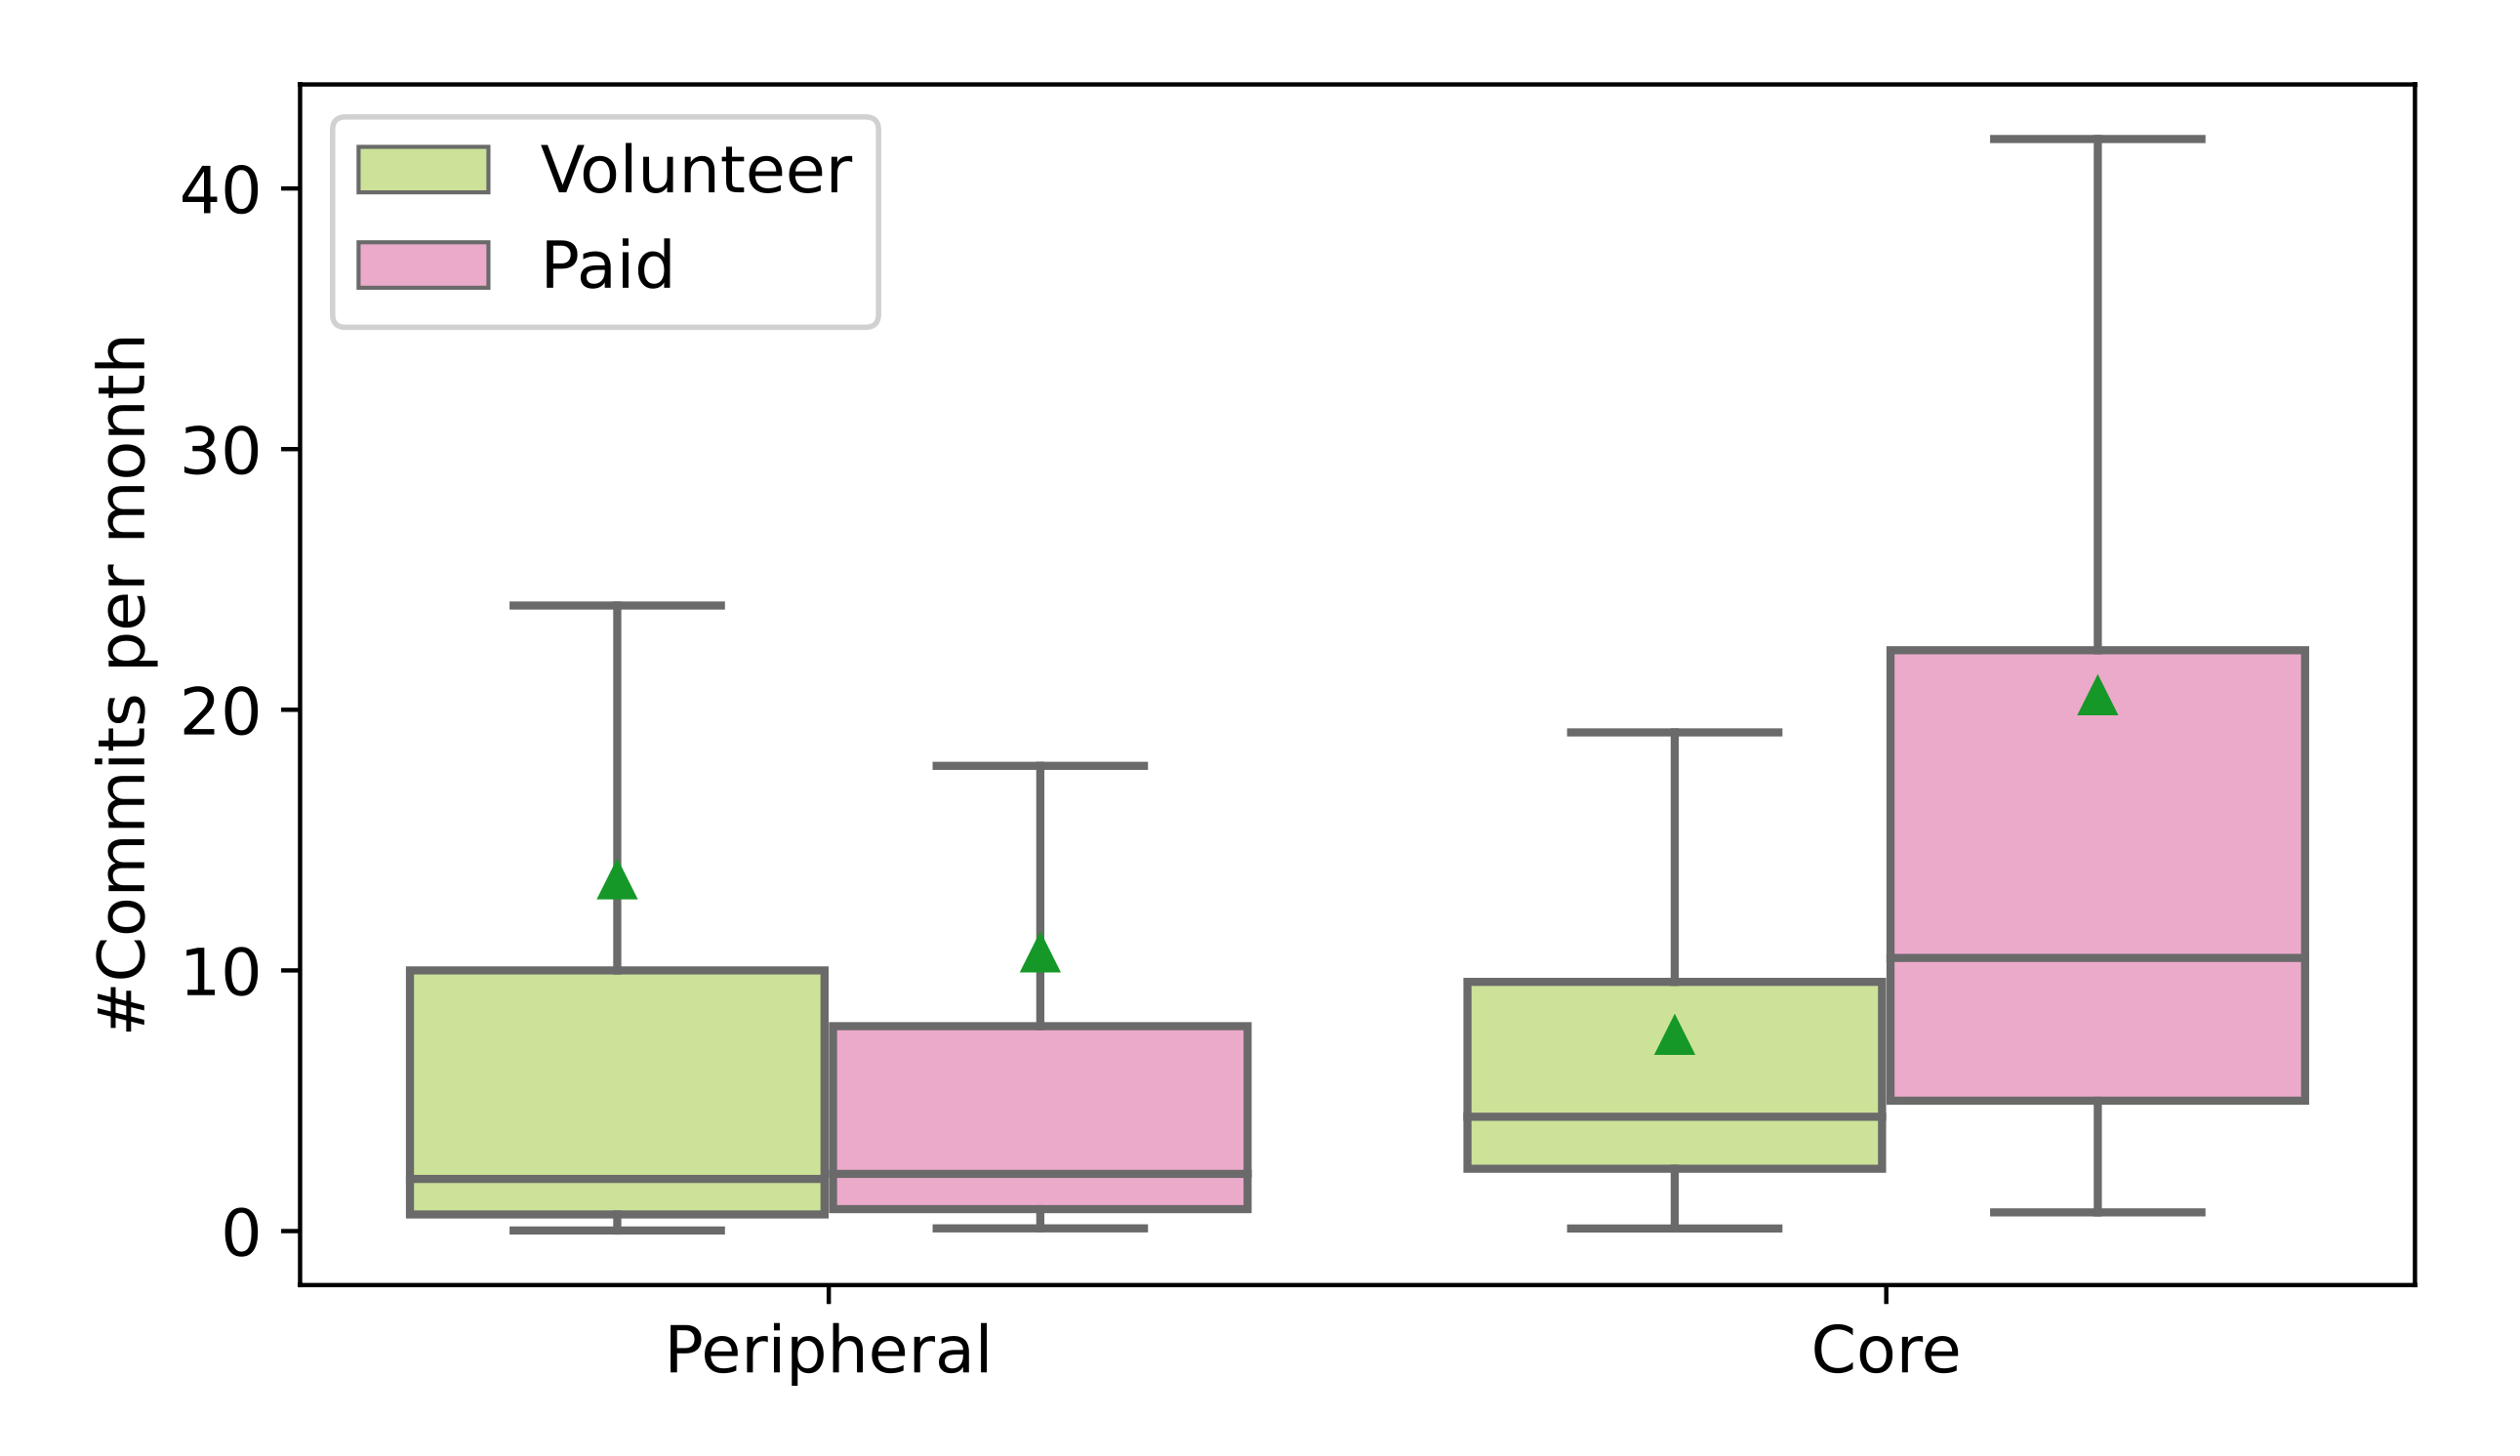
\includegraphics[width=0.65\linewidth]{figs/Contribution_frequency.png}
    \caption{How often paid and volunteer developers contribute to Rust project \citep{08zhang2024paid}}
    \label{fig:contribution_frequency}
\end{figure}


Moreover, commits from one-time paid developers tend to be larger in scope, potentially encompassing more impactful code changes than those of one-time volunteers. This highlights a possible correlation between compensation and the magnitude of contributions. Peripheral paid developers exhibit a higher inclination towards implementing new features compared to unpaid contributors. This trend underscores how financial incentives might influence not only the quantity but also the innovative nature of contributions within the open-source ecosystem.

Collectively, these findings illustrate the complex dynamics of mixed-motivation OSS projects. Understanding these distinctions is crucial for project maintainers seeking to effectively leverage the collaborative potential of both paid and volunteer contributors, ultimately strengthening the sustainability of OSS projects.

4. Role transformation

One of the defining characteristics of OSS projects is the transformation of roles.  Unlike traditional software development models, where users and developers occupy distinct positions, OSS communities blur these lines.  Anyone, from seasoned developers to individuals with technical curiosity, can become a contributor.  This inclusive nature fosters a sense of ownership and empowers users to actively shape the project's evolution.  The potential to transition from user to developer offers a compelling incentive for participation, fostering a community where everyone's voice is valued, and diverse perspectives are encouraged \citep{06ye2003toward,09lakhani2005hackers}.

The progression of OSS systems and communities throughout time is depicted in figure \ref{fig:roleMotivation}.  The responsibilities of developers and users become more entwined as projects expand and mature.  Users who use the program for work-related or personal purposes at first may become active contributors in the future out of a desire to improve the project, take care of certain issues, or impart their knowledge to the community.  This shift in position is evidence of the cooperative spirit of open-source development, where users are empowered to influence the software they use and contribute to a common goal of advancement and innovation.


\begin{figure}[ht]
    \centering
    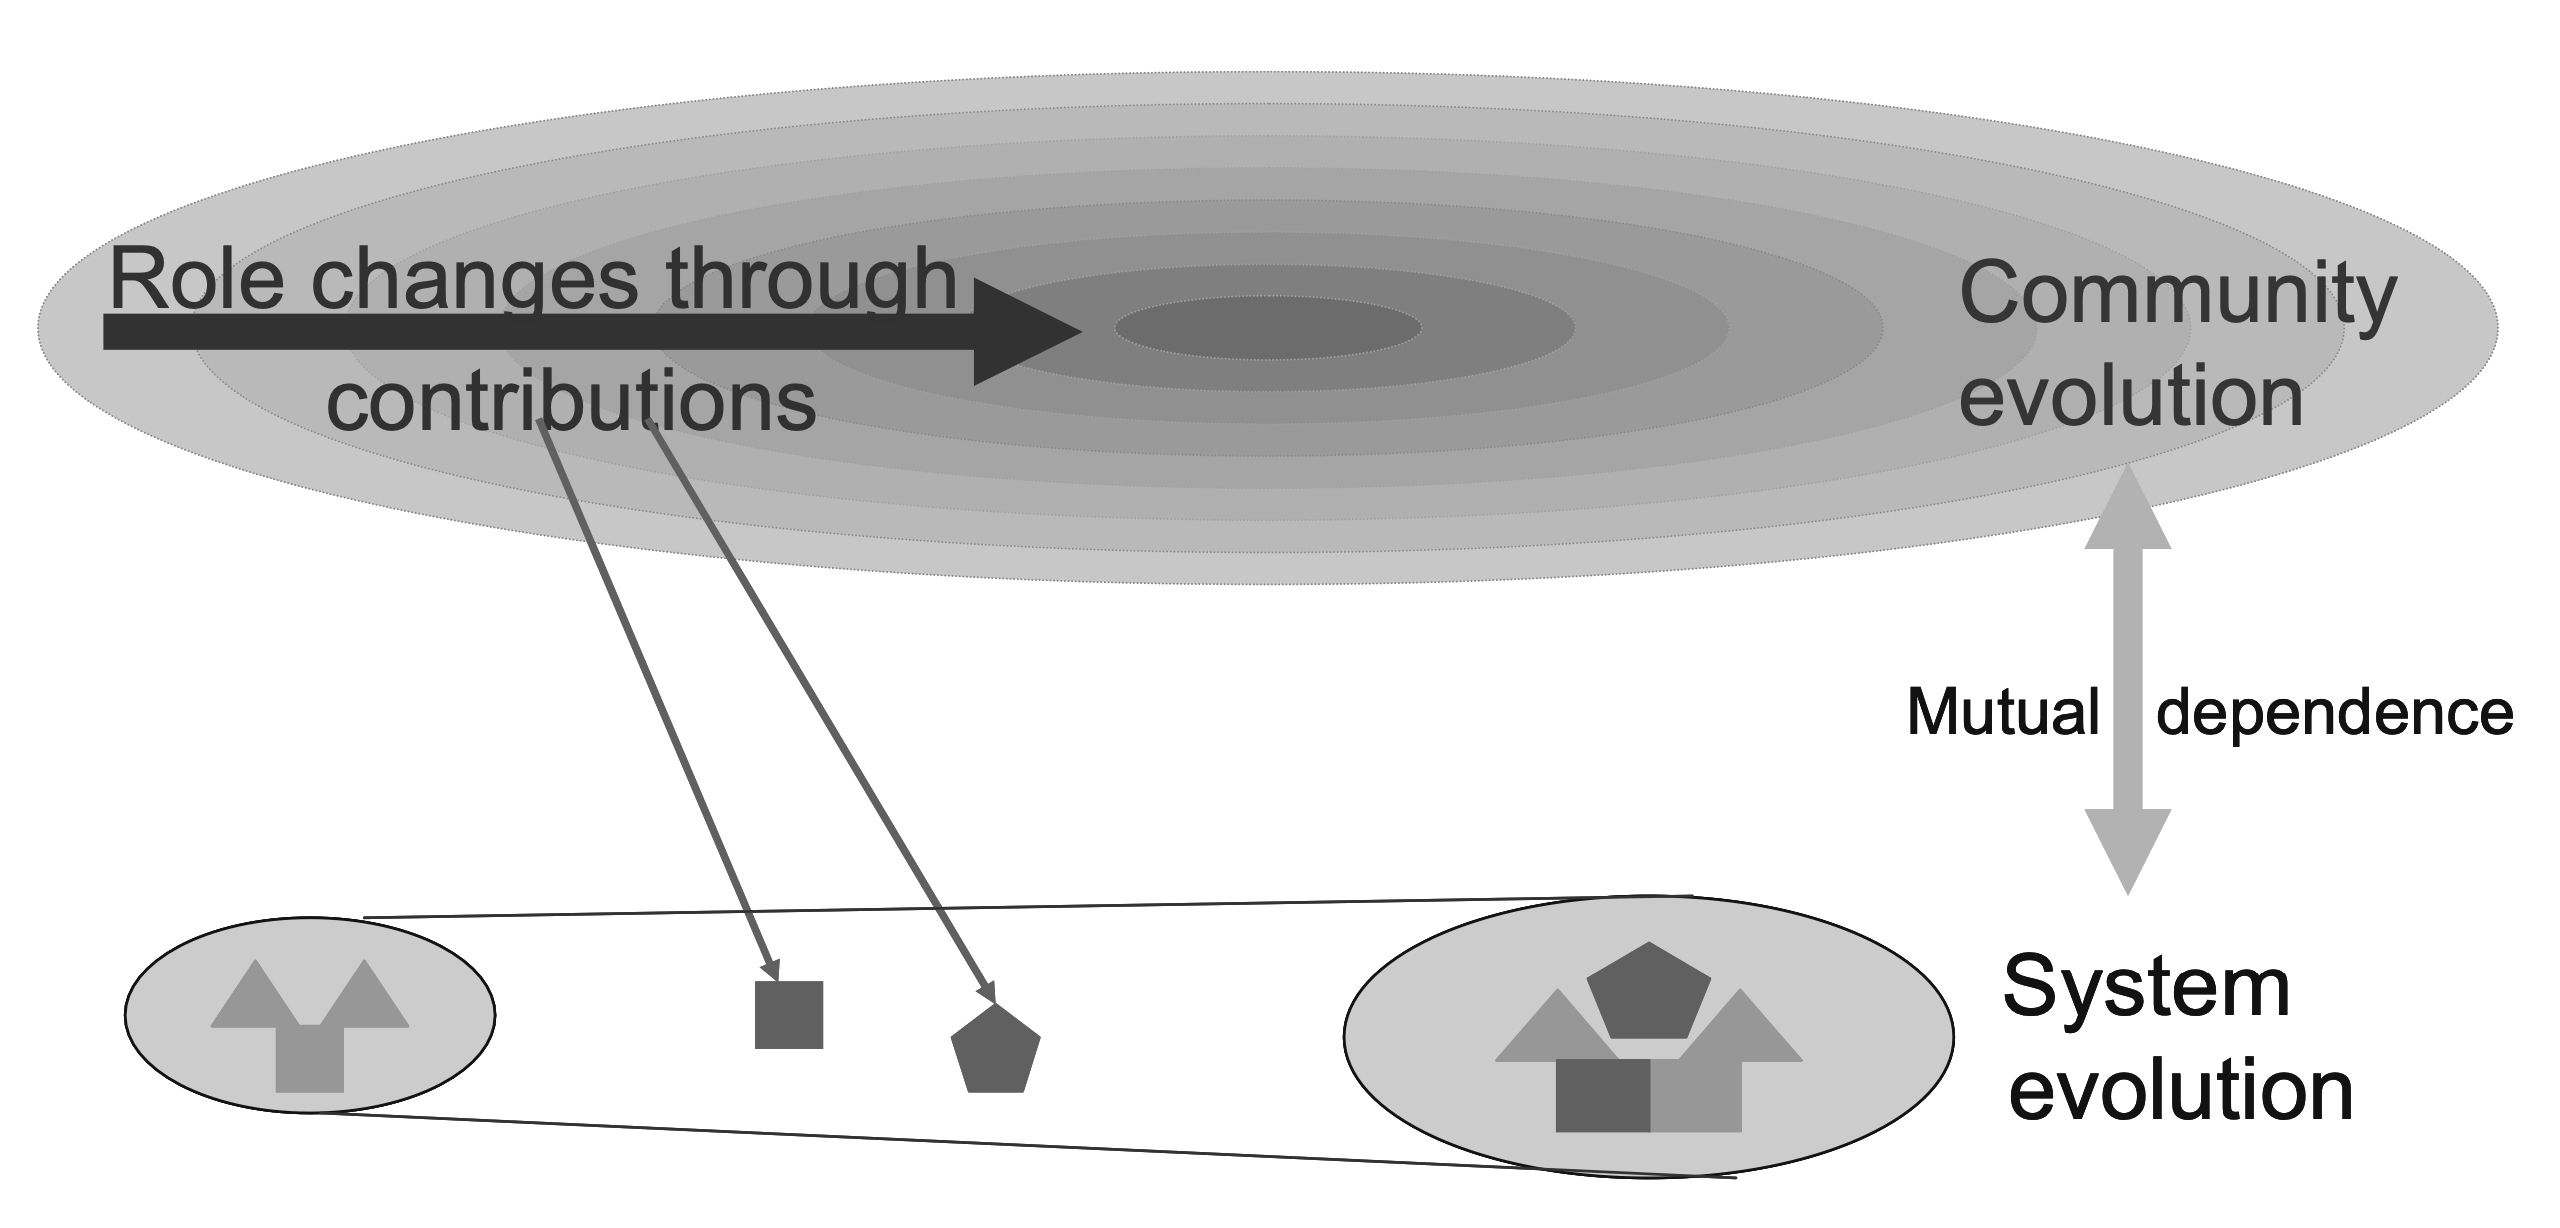
\includegraphics[width=0.65\linewidth]{figs/roleMotivation.png}
    \caption{How open-source software systems and communities grow together \citep{06ye2003toward} }
    \label{fig:roleMotivation}
\end{figure}



Moreover, the opportunity to directly fulfill user needs is a key motivator for developers contributing to open-source projects. Regardless of whether these needs stem from professional or personal pursuits, developers within the OSS community are driven by a desire to create software that tackles real-world challenges and improves user experiences. This direct link between developers and users fosters a collaborative atmosphere where both sides gain from shared knowledge and a commitment to ongoing enhancement.

\subsection{RQ2: Impact of social dynamics}

In addition to investigating the motivations of developers, this research also examined the significant influence of social dynamics on the participation of developers in open-source projects. Through a comprehensive analysis of 13 pertinent studies selected from a pool of over 20 papers, this research has yielded several key findings. These findings highlight the multifaceted nature of developer engagement in open-source initiatives and underscore the importance of social interactions in shaping participation patterns. The subsequent sections will elaborate on these findings, providing a nuanced understanding of the interplay between individual motivations and social forces within the open-source software development ecosystem.

\subsubsection{Community interaction}
The level of interaction within an open-source community is a significant determinant of developer participation. Active communication channels, encompassing forums, mailing lists, and chat platforms, provide essential avenues for collaboration, knowledge sharing, and mutual assistance. These interactions foster a sense of community and belonging, encouraging developers to actively engage with the project and contribute their expertise. Conversely, projects with limited or ineffective communication channels may struggle to attract and retain contributors, as developers may feel isolated or lack the necessary support to make meaningful contributions \citep{05bitzer2007intrinsic,11gerosa2021shifting,20freeman2007material}.


Empirical research consistently demonstrates that developers derive substantial satisfaction from collaborative endeavors and the opportunity to assist others within the open-source ecosystem. Collaboration and teamwork are not merely instrumental means to achieve project goals but are also intrinsically rewarding for developers. The sense of community engendered by open-source projects, along with the opportunity to interact with peers and contribute to a shared endeavor, are integral to the ethos of open-source software development.

The establishment of robust communication infrastructure and feedback mechanisms is paramount for sustaining active developer participation. Clear, transparent, and efficient communication facilitates the resolution of technical issues, the exchange of innovative ideas, and the coordination of efforts among team members \citep{05bitzer2007intrinsic,13li2012leadership}. Moreover, constructive feedback loops enable developers to learn from each other, refine their skills, and enhance the quality of their contributions. Cultivating a supportive and communicative environment fosters a sense of camaraderie and shared purpose, thereby augmenting developer engagement and productivity.

The integration of social features within open-source platforms, such as mechanisms for connecting individuals seeking assistance with those willing to provide it, can substantially enhance community interactions and support. The open-source ethos is intrinsically predicated on collaboration and the open exchange of knowledge, and social platforms facilitate these interactions by creating virtual spaces for developers to connect, communicate, and collaborate. The sense of belonging to a community of like-minded individuals fosters camaraderie, mutual assistance, and a shared sense of purpose, all of which contribute to sustained engagement and project success.

In order to encourage engagement and retention in open-source communities, it is imperative that seasoned developers be present and eager to assist beginners. Mentorship programs enable inexperienced developers to overcome obstacles, learn new skills, and blend in with the community by offering them priceless advice, support, and encouragement. This knowledge transfer across generations is critical to the long-term viability and expansion of open-source initiatives. Open-source communities may draw and keep a wide range of contributors by creating a warm, accepting atmosphere that values knowledge sharing and mentoring. This ensures the ongoing creativity and vitality of the open-source software ecosystem.



\subsubsection{Networking opportunities}
Novice contributors often transition their initial motivations towards career-oriented goals, leveraging open-source projects as a portfolio to showcase their skills to potential employers \citep{05bitzer2007intrinsic,11gerosa2021shifting}. Participation in these projects offers invaluable networking opportunities, fostering connections with industry professionals and paving the way for career advancement \citep{10wu2007empirical,11gerosa2021shifting,13li2012leadership}. By demonstrating their expertise and building a reputation within the open-source community, developers can attract job offers, consulting opportunities, and further professional development. Moreover, the open-source environment allows developers to gain experience with diverse technologies, tools, and methodologies, broadening their skillset and making them more adaptable to the evolving demands of the tech industry.

Open-source projects serve as a platform for developers to connect with industry peers, experts, and potential employers \citep{10wu2007empirical,11gerosa2021shifting,13li2012leadership}. These connections can lead to collaborations on new projects, expanding professional networks and opening doors to career growth opportunities. The collaborative nature of open-source projects allows developers to establish relationships with like-minded individuals, fostering a supportive community that encourages knowledge sharing and mutual growth.  Additionally, engaging with established open-source communities can provide developers with exposure to industry best practices, coding standards, and project management methodologies, further enhancing their professional capabilities.

Open-source projects are inherently collaborative environments, providing developers with ample opportunities to share knowledge, learn from others, and enhance their skills. The exchange of ideas, feedback on code, and exposure to diverse perspectives within the community foster continuous learning and skill improvement. Through interactions with other developers, mentorship, and exposure to new ideas and technologies, developers are motivated to stay engaged and contribute to the project's ongoing success \citep{05bitzer2007intrinsic,06ye2003toward,09lakhani2005hackers,13li2012leadership}. This culture of continuous learning and knowledge sharing also helps developers stay abreast of the latest trends and innovations in the tech industry, ensuring their skills remain relevant and in demand.


\subsubsection{Community culture and support }

Engaged and supportive open-source communities act as a catalyst for developer contributions by offering assistance, constructive feedback, and a sense of belonging. This collaborative atmosphere nurtures knowledge sharing, mutual support, and a strong sense of community among developers. Ultimately, positive social interactions and a supportive environment within these communities drive increased motivation and sustained engagement among developers. \citep{10wu2007empirical,12choi2015characteristics,13li2012leadership,16ke2008motivations}.

Social coding platforms have revolutionized the open-source landscape, shifting the culture from its traditional hacker-centric roots to a more inclusive, collaborative community. By lowering barriers to entry, these platforms have made open-source projects more accessible and welcoming to newcomers, regardless of their technical expertise \citep{06ye2003toward,11gerosa2021shifting}. They foster a sense of belonging and encourage participation through features like issue tracking, discussion forums, and code review tools, promoting knowledge sharing and collaborative problem-solving. This cultural shift has not only broadened the pool of contributors but has also led to more diverse perspectives and innovative solutions within the open-source ecosystem.

Roles within OSS communities are dynamic and fluid, allowing members to assume greater responsibilities by contributing meaningfully to projects. As individuals transition between roles, they actively influence the social dynamics and structure of the community, ultimately driving its evolution \citep{06ye2003toward}. This flexibility enables OSS communities to adapt and thrive in response to the evolving needs of projects and the diverse contributions of their members.


Open-source platforms that promote collaboration and offer diverse avenues for appreciation, ranging from formal accolades to informal gestures like awarding stars to projects, significantly enhance the sense of belonging and recognition among community members. Active engagement in these communities allows developers to gain recognition for their contributions, cultivate a positive reputation, and establish a personal brand within the wider developer community \citep{11gerosa2021shifting,13li2012leadership}.

The paper "OpenRank Leaderboard: Motivating Open Source Collaborations Through Social Network Evaluation in Alibaba" presents a study conducted to explore the impact of the OpenRank Leaderboard on open source collaborations within Alibaba's projects \citep{07zhao2024openrank}. The research methodology involved a mixed-methods approach, including case studies, surveys, analysis of project metrics data, semi-structured interviews, and thematic coding. The study focused on seven open source projects initiated by Alibaba, aiming to investigate how gamified leaderboards can motivate collaboration and drive innovation in software development.

\begin{figure}[ht]
    \centering
    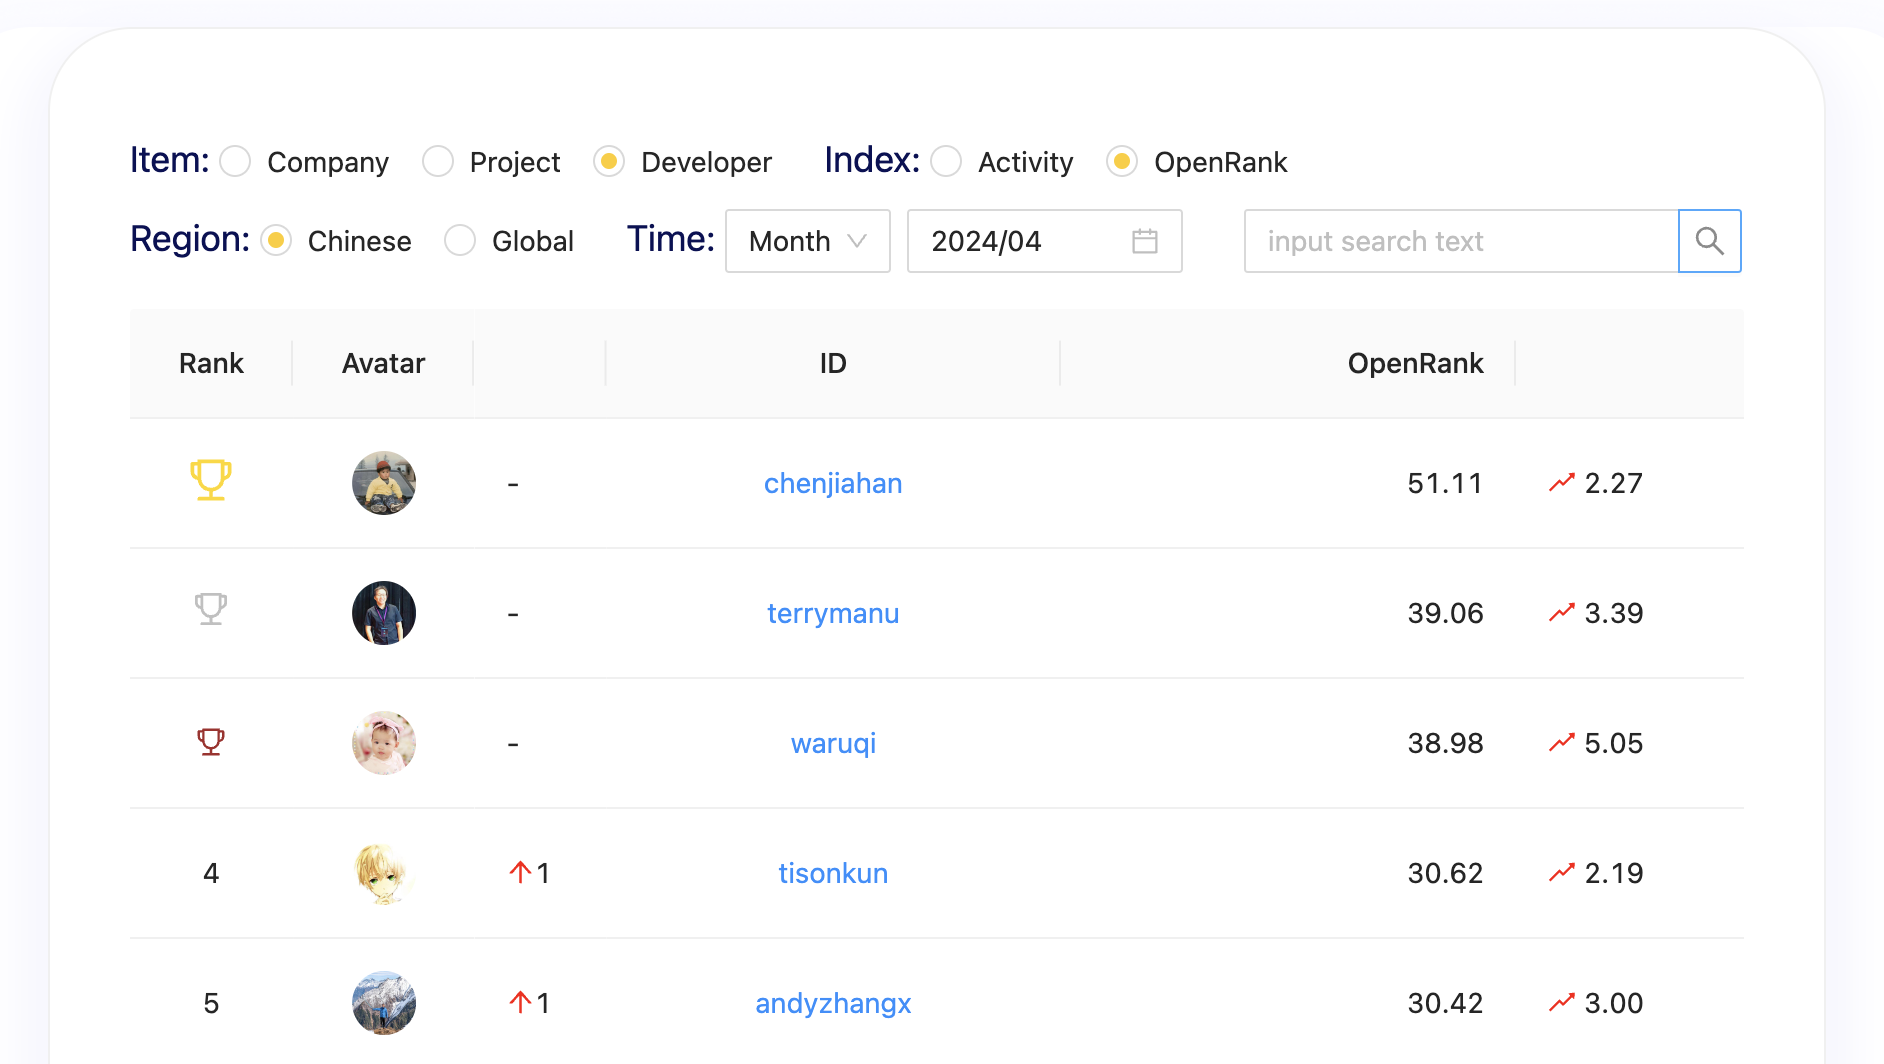
\includegraphics[width=0.85\linewidth]{figs/openrank.png}
    \caption{A screenshot of the interface of the OpenRank Leaderboard in May, 2024}
    \label{fig:openrank}
\end{figure}



Through the implementation of the OpenRank Leaderboard, the study found that developers were motivated to engage in more transparent communication, leading to improved collaboration behavior and a better community atmosphere. The leaderboard incentivized developers to make smaller, independent \ac{pr} and avoid direct commits to the repository, ultimately enhancing the quality of code contributions and fostering continuous improvement within the projects. The research also highlighted the role of the leaderboard in promoting healthy competition among developers, encouraging sustained engagement, and driving innovation within the open source projects.

The findings of the study indicated that the OpenRank Leaderboard effectively evaluates and steers developers' contributions, leading to positive behavioral changes and enhanced collaboration habits. Developers expressed a favorable perception of using graph network algorithms for contribution evaluation, with many acknowledging the alignment of rankings with their community perceptions and the value of combining results with community incentive operations. Overall, the study contributes valuable insights into the impacts and perceptions of using leaderboards as a gamification mechanism in company-led open source projects, emphasizing the importance of social network evaluation in motivating open source collaborations and driving innovation in software development.


\subsection{RQ3: Contribution barriers}

Beyond examining the motivations and social dynamics that propel developer participation in open-source projects, this research also delved into the barriers hindering their contributions. Through an analysis of five selected studies, several key challenges were identified that impede developer engagement and limit their ability to contribute effectively. The following sections will explore these barriers in detail, providing a comprehensive overview of the obstacles developers face in the open-source software development landscape. Based on a previous study by Mariam \citep{04guizani2021long}, the barriers to contribution were categorized into three main categories: technical challenges, social challenges, and process challenges. Each category encompasses distinct obstacles that hinder developer participation and require targeted interventions to overcome.


The chart \ref{fig:barriers} illustrates the obstacles individuals encounter when contributing to open source software projects which was found in 5 papers. The most frequent challenges revolve around social interaction, lack of timely responses or support, and technical difficulties, each occurring four times. Feeling intimidated or shy, cultural differences, and uncertainty about where to begin are also notable challenges, each happening twice. Other obstacles like submission procedures, governance compliance difficulties, unmet expectations, reception issues, inadequate or outdated projects, and prior technical experience are less common, each occurring once.

\begin{figure}[ht]
    \centering
    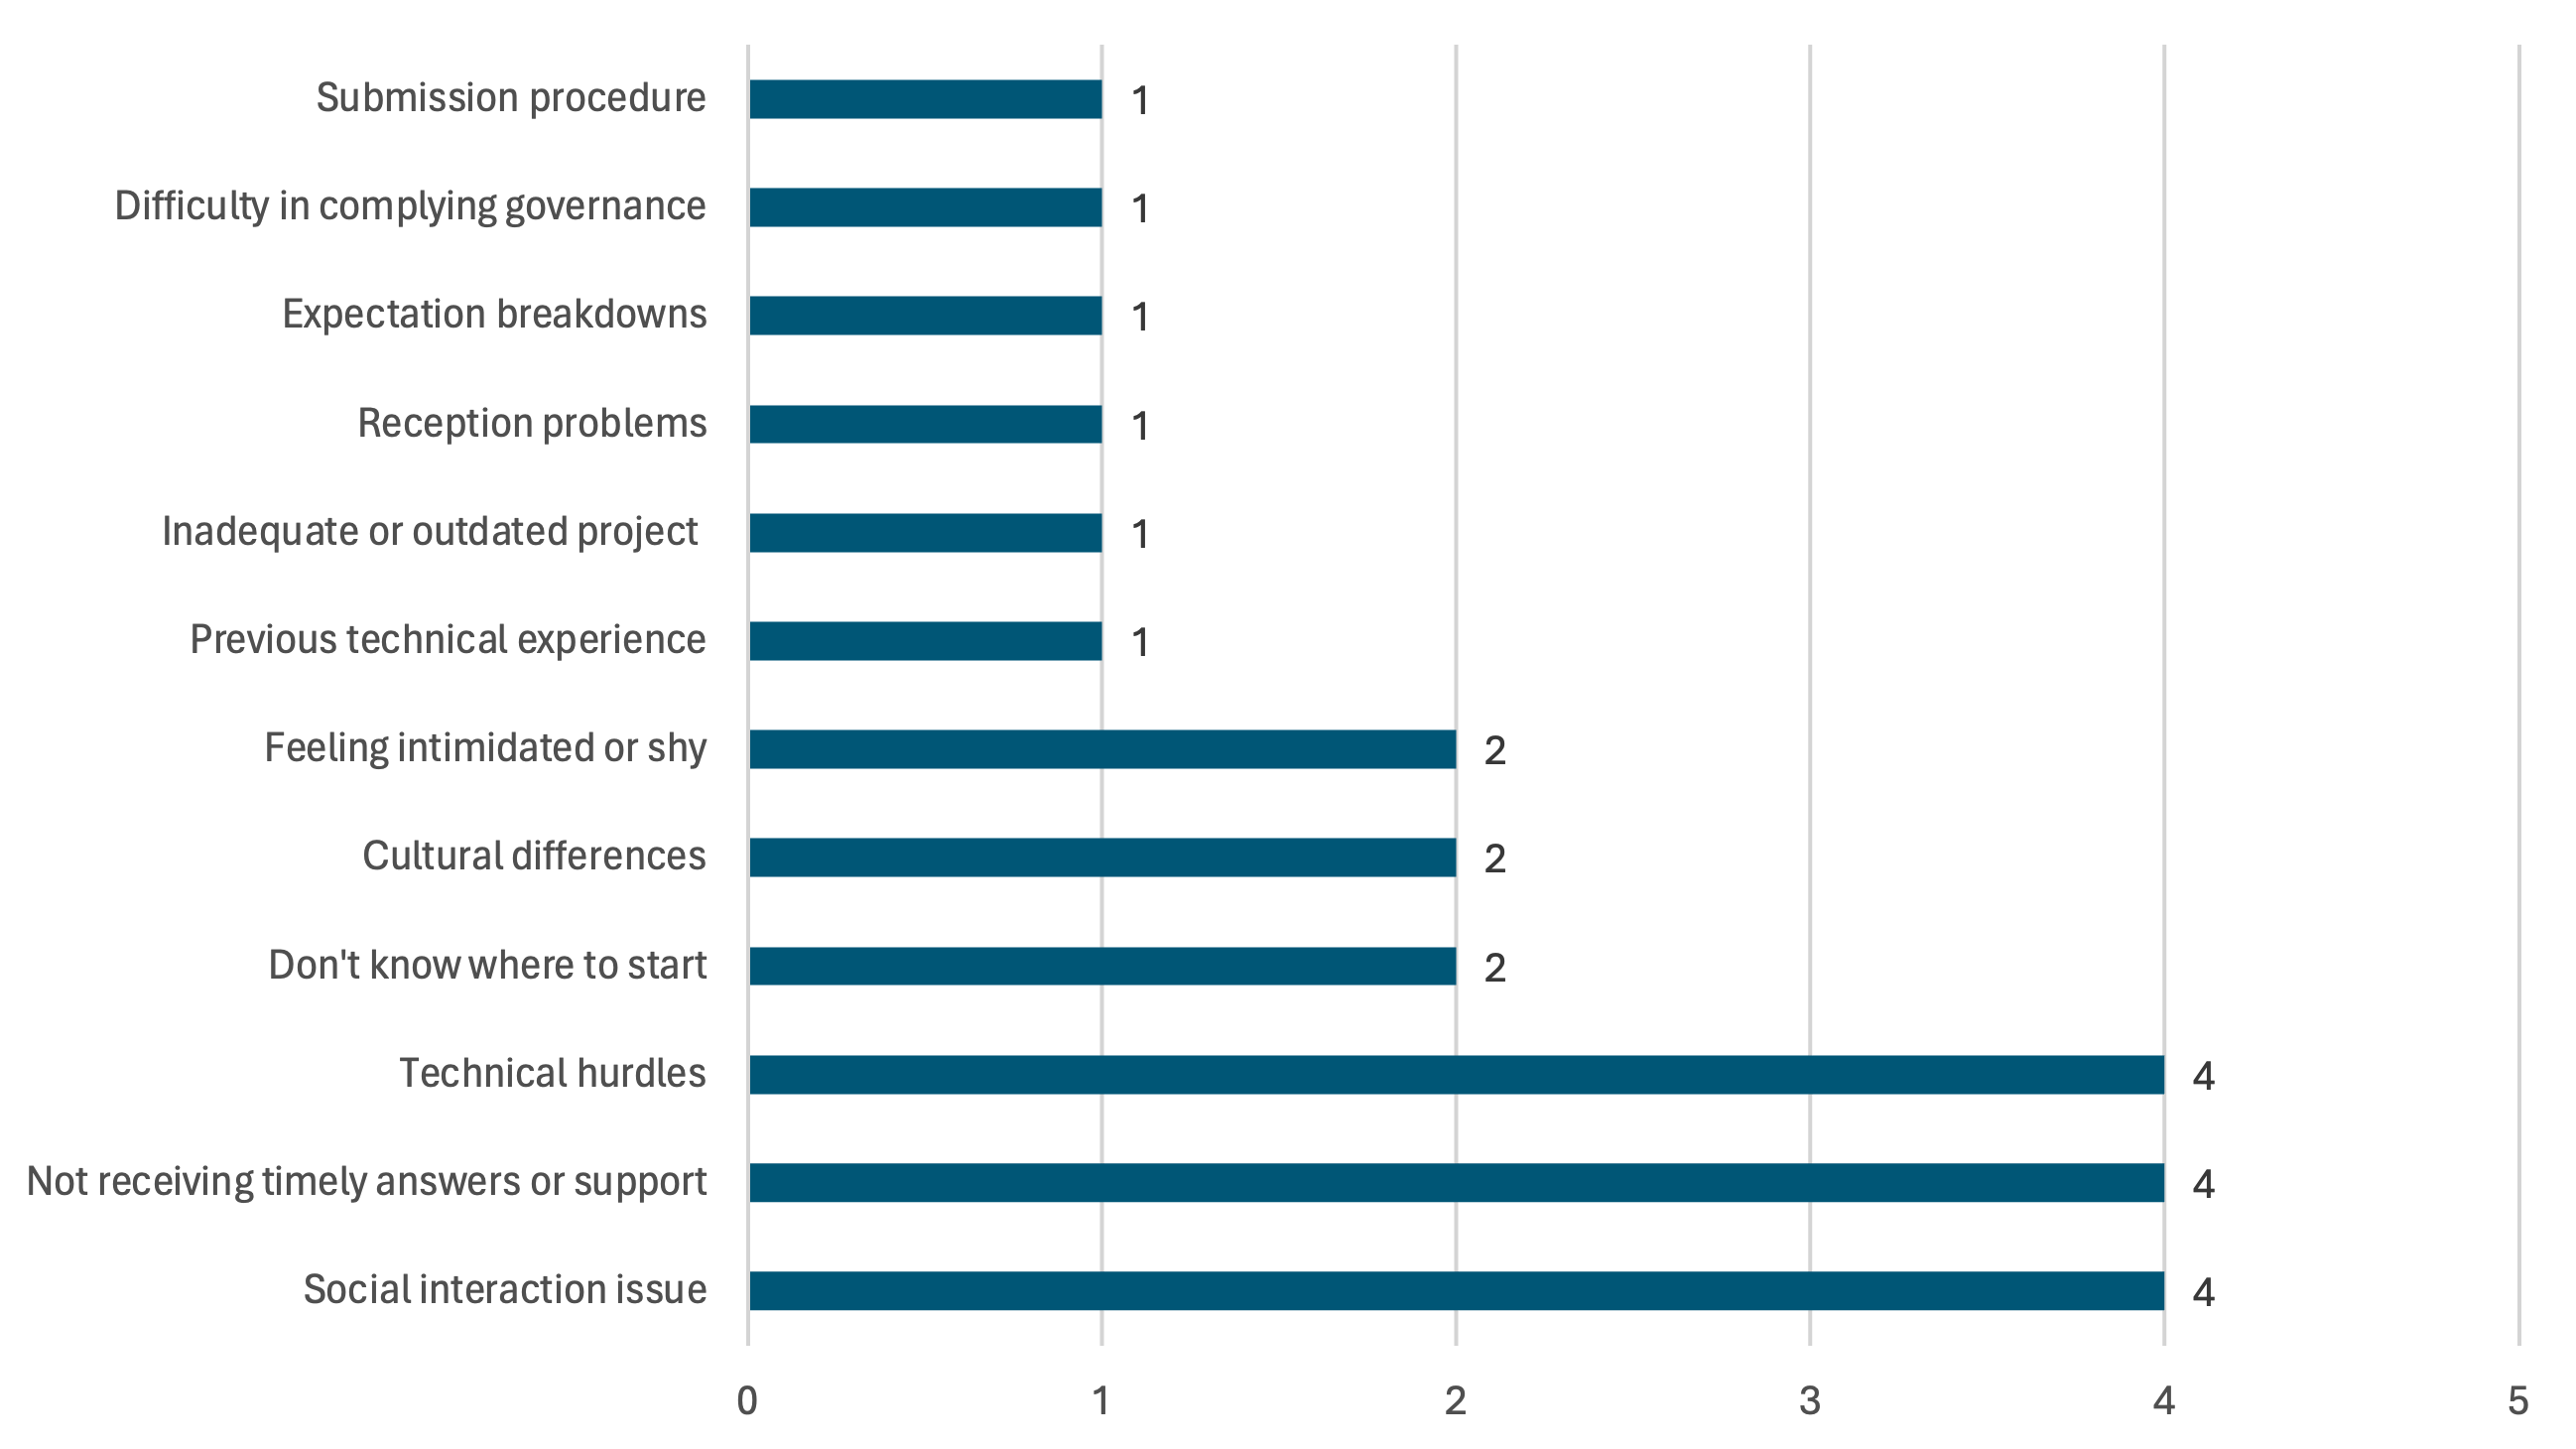
\includegraphics[width=1\linewidth]{figs/barriers.png}
    \caption{Barriers to contributing to open-source software projects}
    \label{fig:barriers}
\end{figure}



\subsubsection{Technical challenges}

A significant technical barrier to open-source contribution is the lack of technical background and domain expertise among potential contributors. Without a foundational understanding of the project's technological underpinnings, whether it's a specific programming language, framework, or software architecture, individuals may struggle to effectively engage and contribute to its development. Additionally, a lack of domain expertise in the subject matter the project addresses can hinder understanding of the problem space and the proposed solutions, making it difficult to provide meaningful contributions.

\begin{figure}[ht]
    \centering
    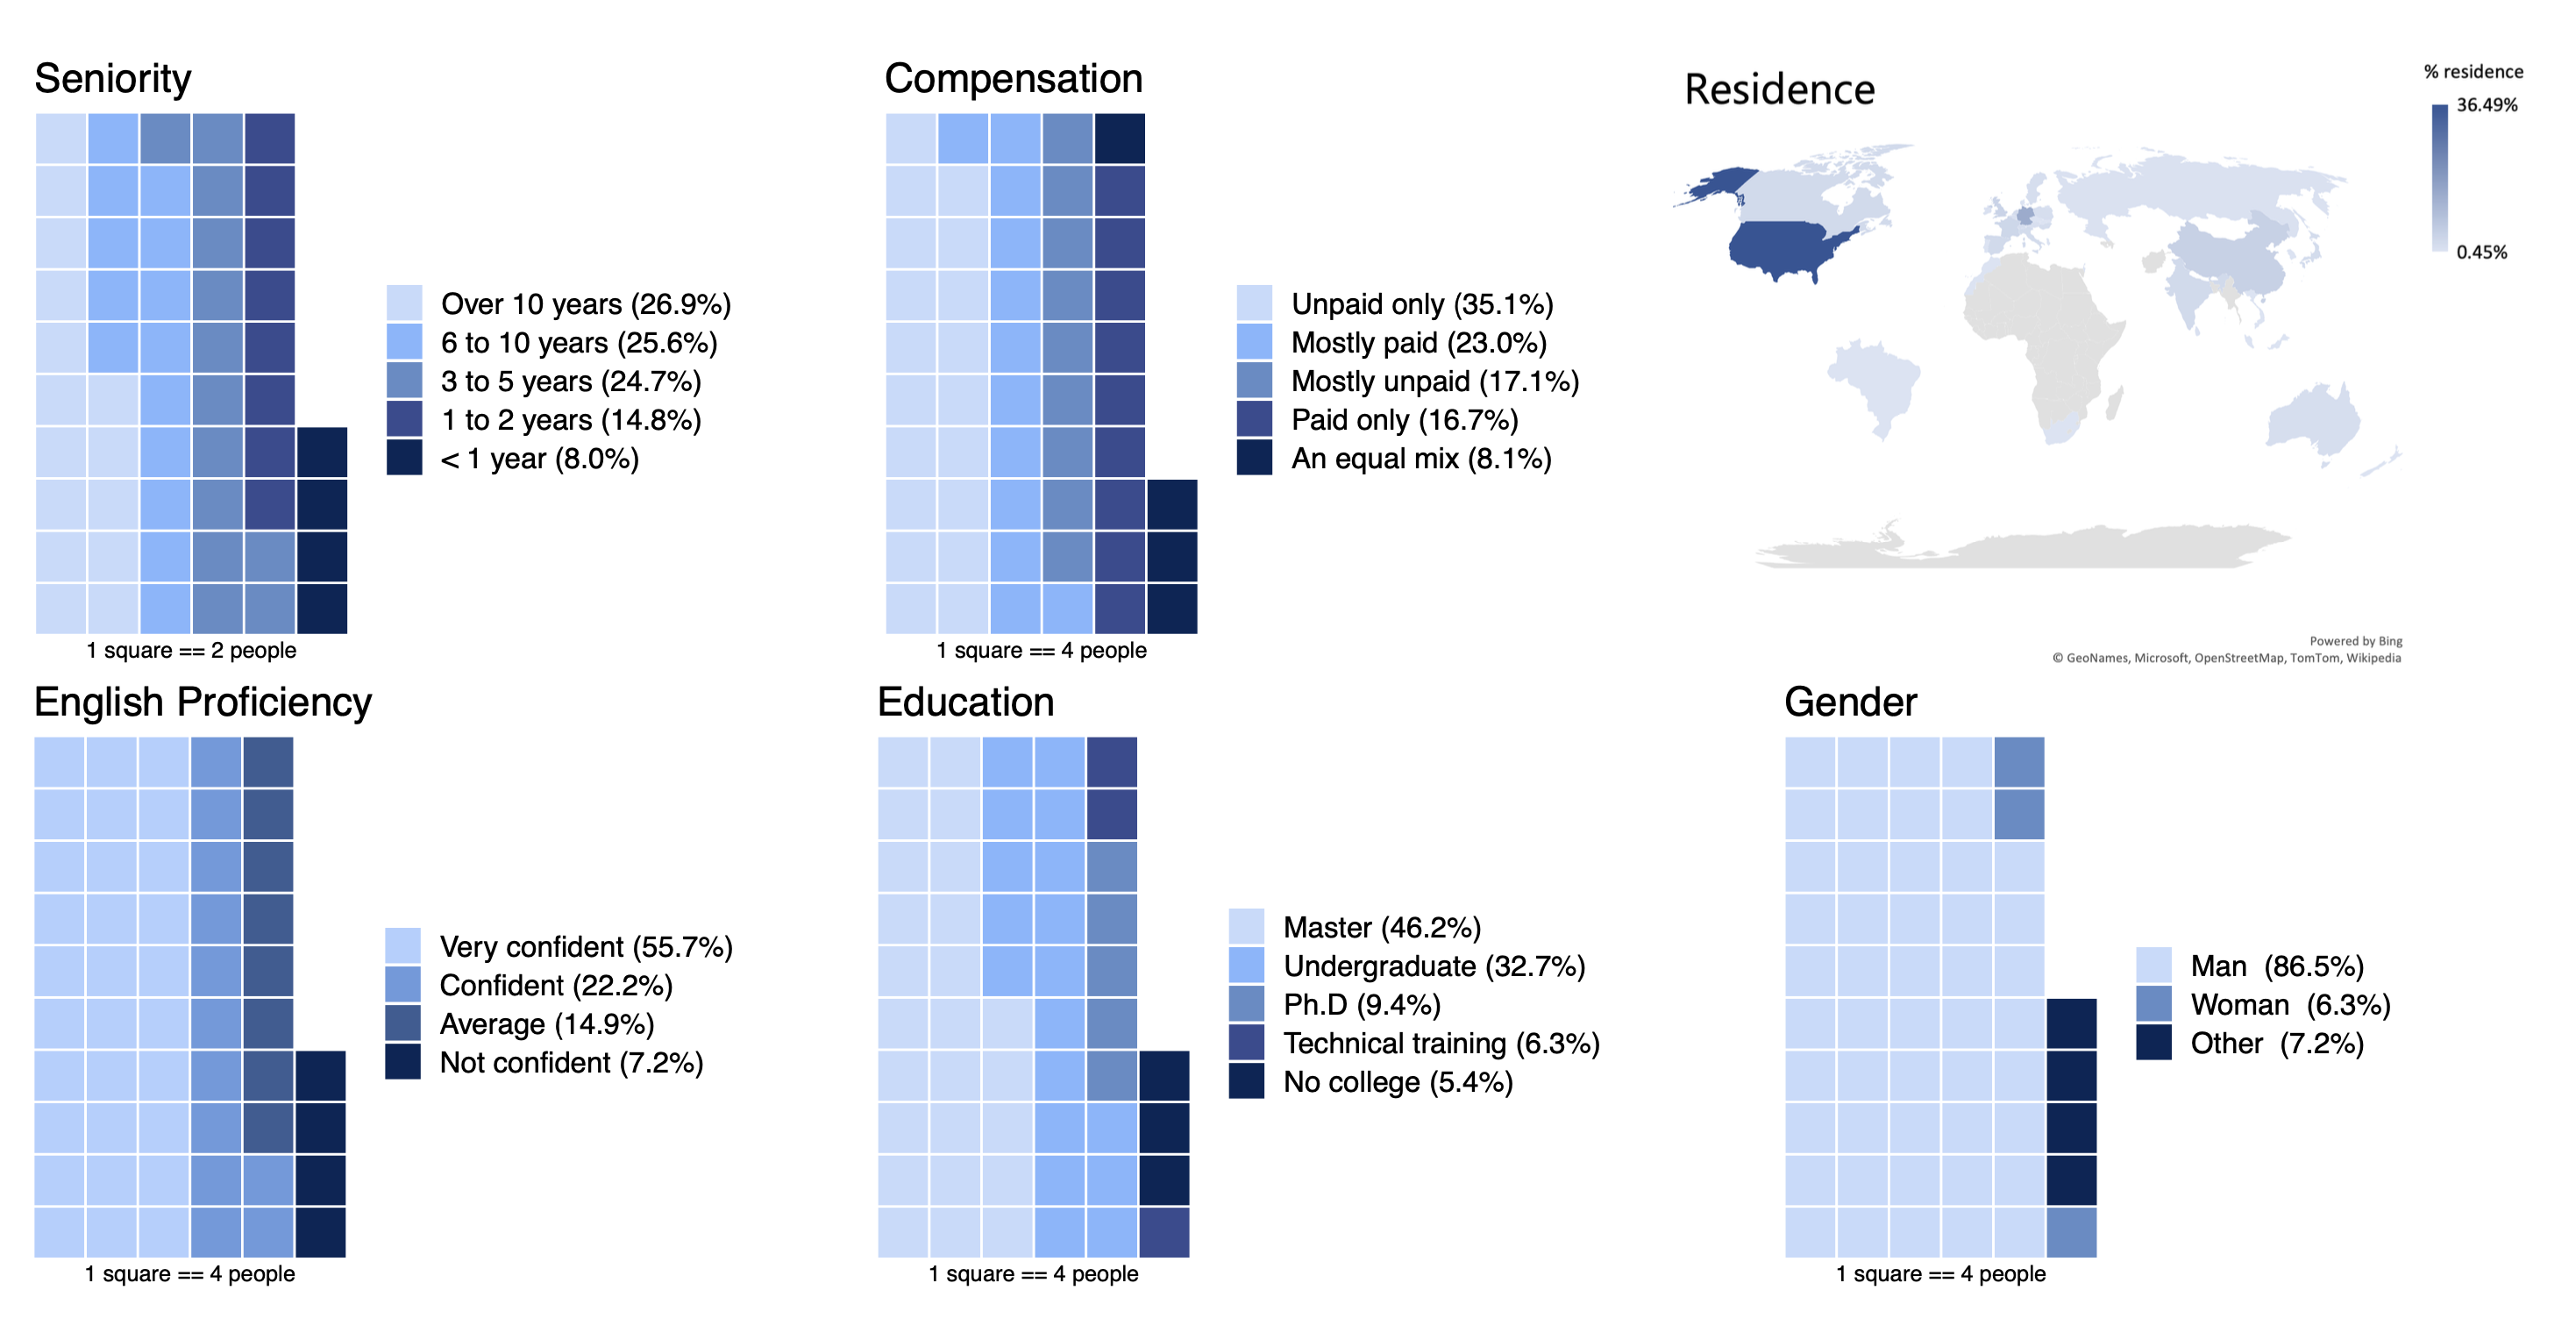
\includegraphics[width=1\linewidth]{figs/contributor_background.png}
    \caption{The background of the 223 developers from \ac{asf} \citep{04guizani2021long}}
    \label{fig:contributor_background}
\end{figure}

The diversity of programming languages used within and across open-source projects presents another challenge. Many projects utilize multiple languages for different components, and the open-source ecosystem as a whole encompasses a vast array of programming languages. Contributors often need to familiarize themselves with these languages to effectively understand and modify code, which can be daunting and time-consuming, particularly for those with limited programming experience or those accustomed to a single language.


Becoming a contributing member of an OSS project often entails acquiring project-specific skills, a process that can span months to a year. This temporal investment is highlighted in \citet{bird2007open} analysis of three OSS projects, where the median duration for newcomers to submit their initial patch and subsequently gain acceptance was revealed. This underscores the significant commitment required to successfully integrate into and contribute to OSS projects. The figure \ref{fig:timeskill} illustrates the time required to learn skills particular to a project, emphasizing the steep learning curve faced by newcomers.

\begin{figure}[ht]
    \centering
    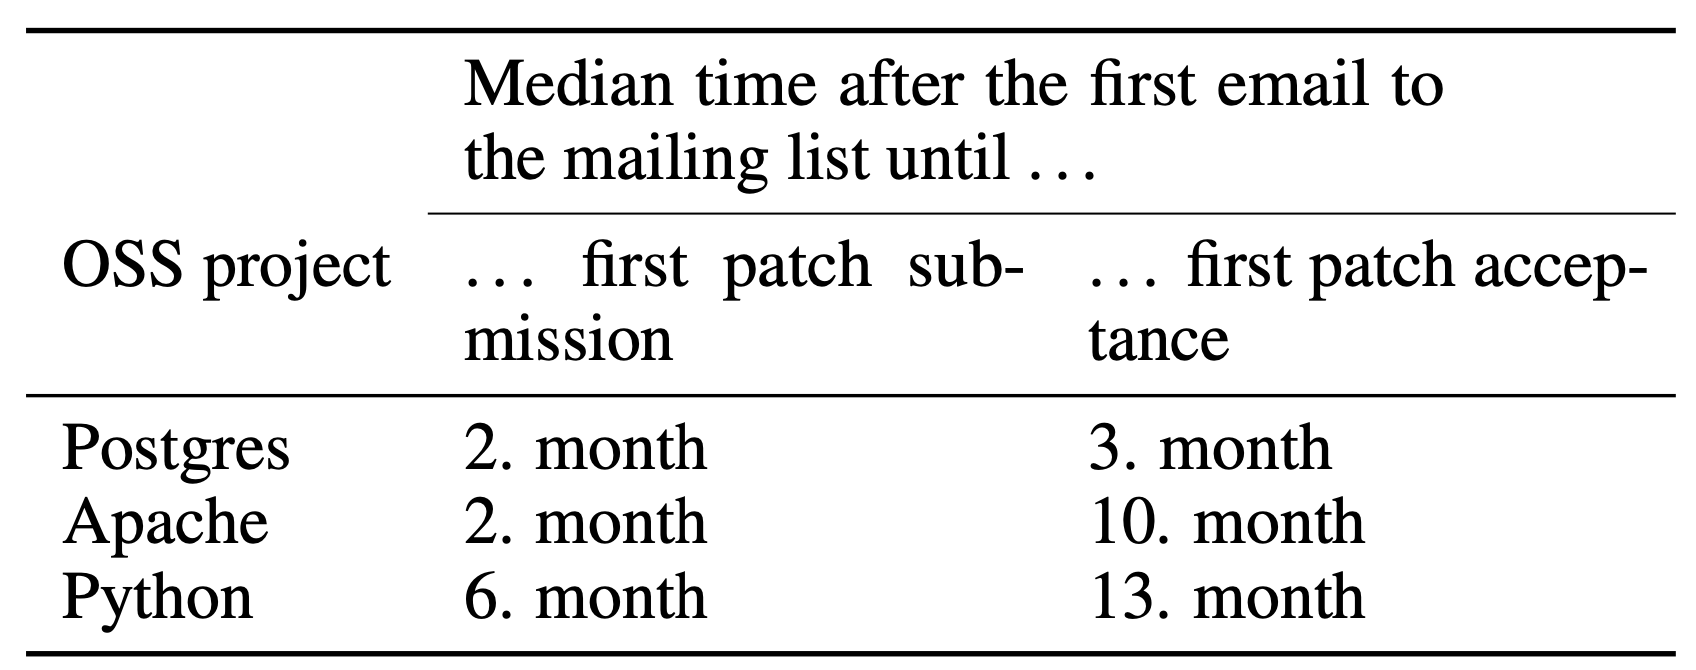
\includegraphics[width=0.65\linewidth]{figs/timeskill.png}
    \caption{Time required to learn skills particular to a project \citep{bird2007open}}
    \label{fig:timeskill}
\end{figure}

Discrepancies in technical skills and knowledge backgrounds among contributors can create a challenging environment for newcomers \citep{01steinmacher2015systematic,04guizani2021long}. Open-source projects often attract individuals with varying levels of expertise, from seasoned developers to those just starting their coding journey. Navigating a project with such diverse skill levels can be intimidating, making it difficult for newcomers to find their footing, ask questions without feeling inadequate, and contribute meaningfully \citep{14hannebauer2017relationship}.

Inadequate or outdated project documentation further compounds the challenges faced by contributors. Clear, comprehensive, and up-to-date documentation is crucial for understanding the project's codebase, workflow, and contribution guidelines. It serves as a roadmap for new contributors, guiding them through the project's intricacies. Without well-maintained documentation, newcomers may struggle to locate the correct areas for modification, understand the reasoning behind existing code, and follow established conventions, ultimately hindering their ability to contribute effectively to the project's development.



\subsubsection{Social challenges}

Effective communication is paramount in the open-source landscape, yet it is often fraught with challenges that can impede participation and collaboration. Limitations in the available communication tools, such as reliance on text-based platforms or asynchronous communication channels, can hinder real-time interaction and create misunderstandings. Additionally, diverse communication styles among members, ranging from direct and concise to more elaborate and nuanced, can lead to misinterpretations and impede the development of shared understanding. Moreover, conflicting viewpoints and disagreements within the community, while natural, can escalate into unproductive debates that alienate newcomers and create an unwelcoming environment \citep{02steinmacher2015social}.

% Image
\begin{figure}[ht]
    \centering
    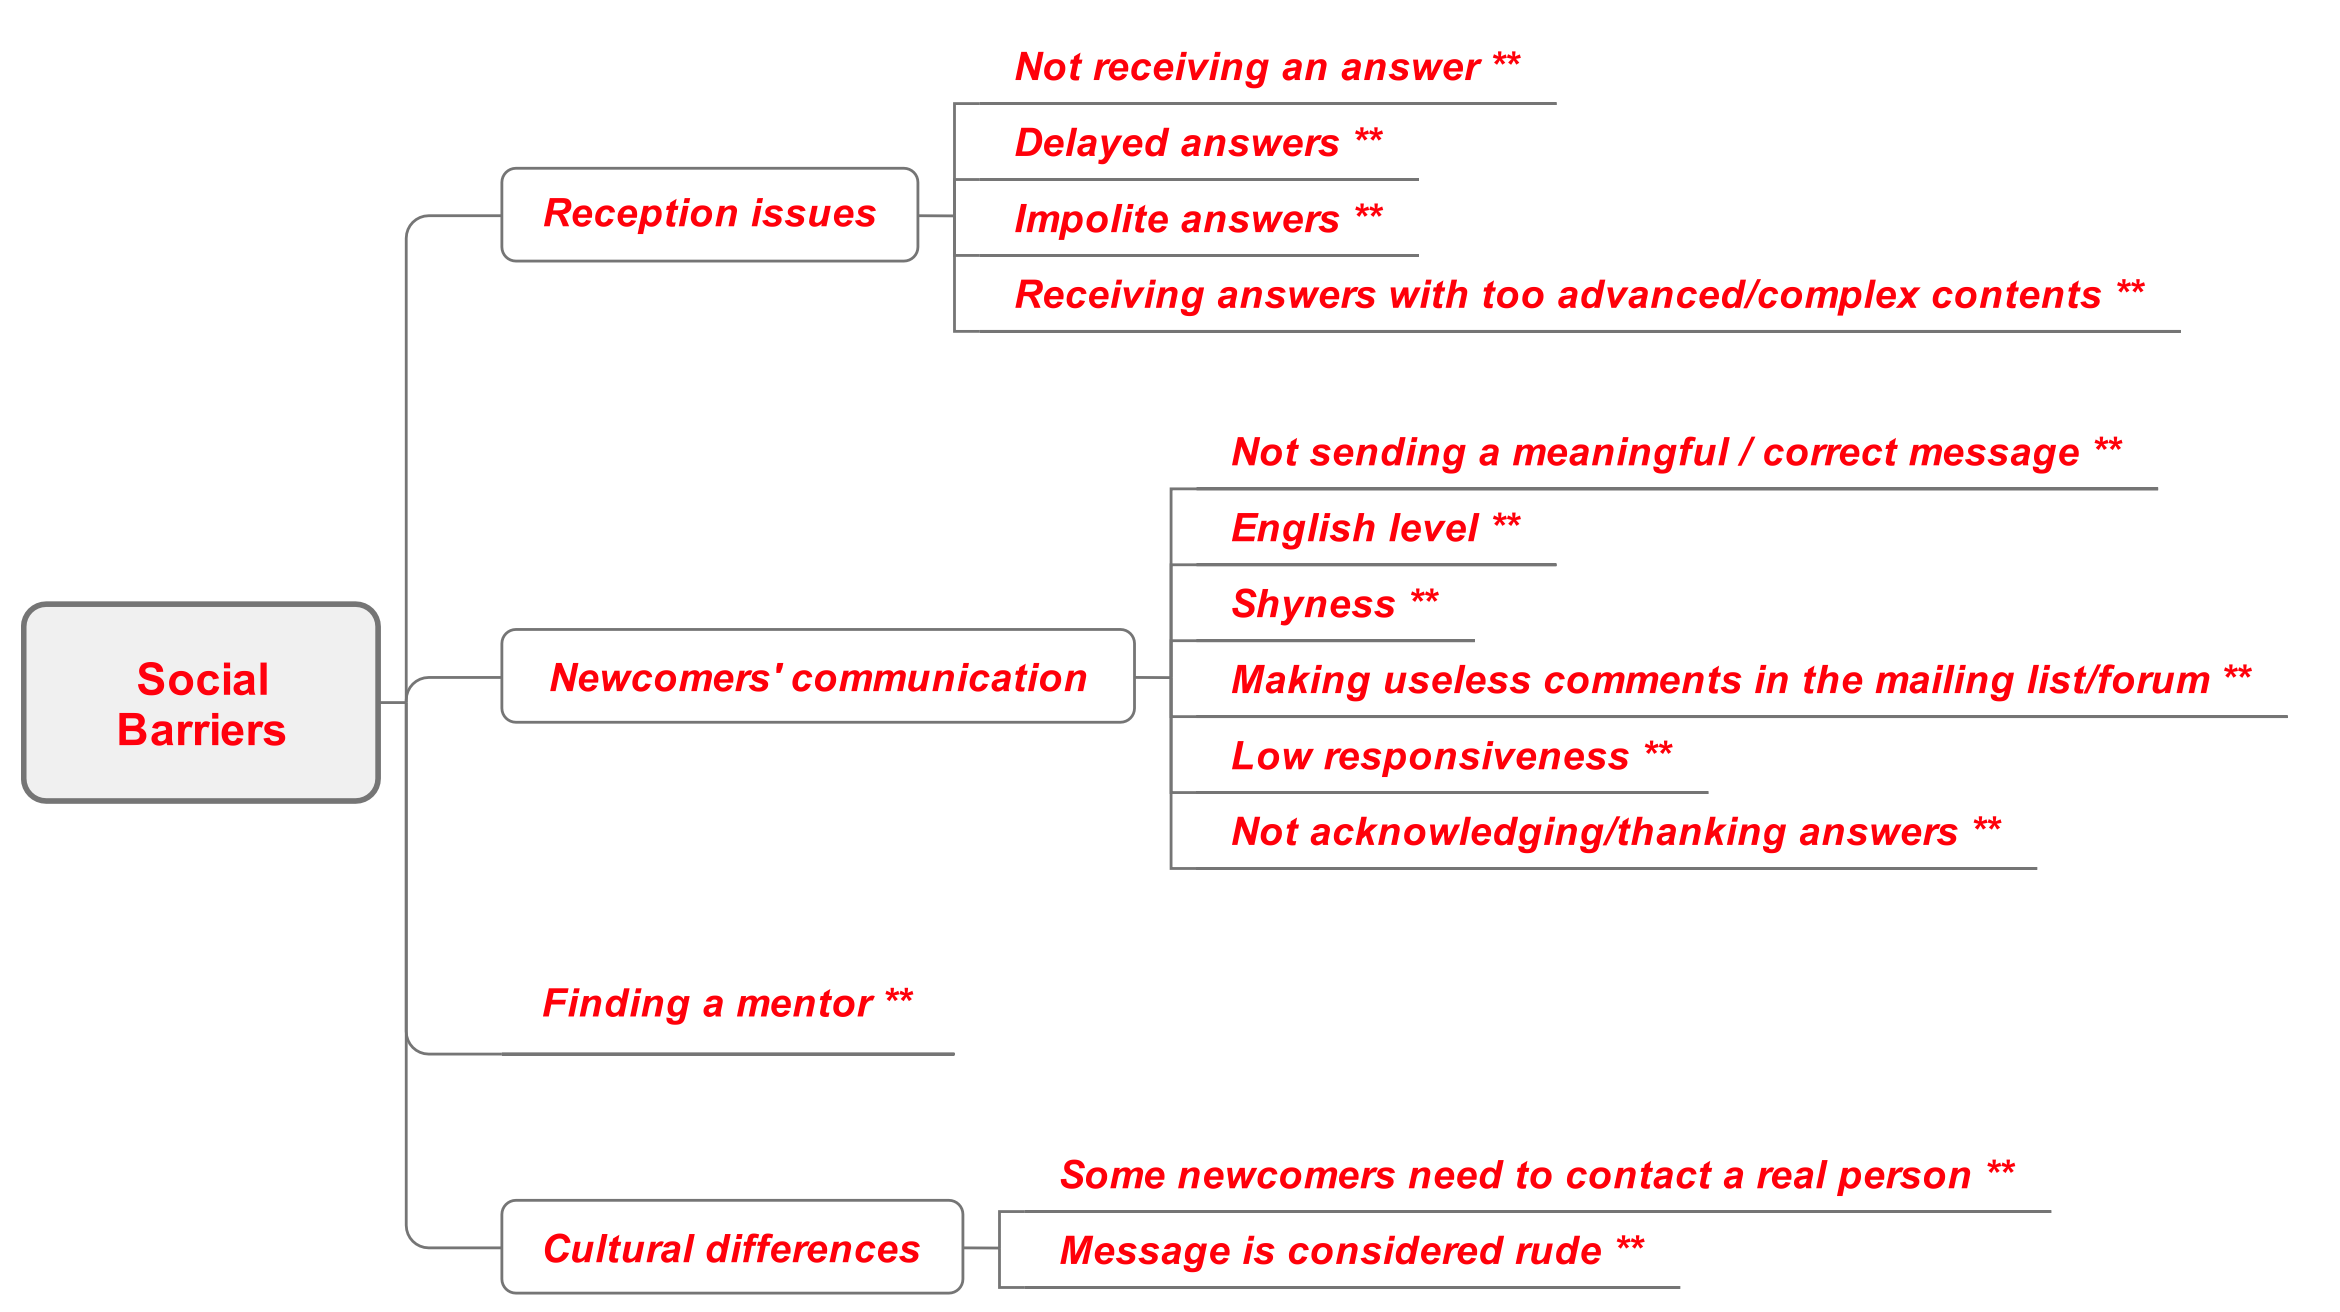
\includegraphics[width=1\linewidth]{figs/socialbarrier.png}
    \caption{Social barriers from Steinmacher's study \citep{03steinmacher2019overcoming}}
    \label{fig:socialbarrier}
\end{figure}

The social dimension of open-source projects is equally crucial, as it fosters a sense of belonging and encourages collaboration. However, newcomers often encounter difficulties establishing connections with project members, particularly in large and established communities. This can lead to feelings of isolation and a lack of mentorship or guidance, making it challenging to navigate the project's intricacies and identify suitable contribution opportunities. Moreover, if newcomers perceive a lack of responsiveness or support from existing members, their enthusiasm may wane, and they may ultimately abandon their efforts \citep{01steinmacher2015systematic,02steinmacher2015social,03steinmacher2019overcoming,04guizani2021long,14hannebauer2017relationship}.

The responsiveness of the community is a critical determinant of newcomers' experiences and long-term engagement. When individuals feel that their questions are ignored, their contributions are not acknowledged, or their efforts are not valued, they may become demotivated and disengage from the project. Conversely, timely feedback, recognition, and support can boost morale and encourage continued participation. Therefore, fostering a culture of responsiveness and inclusivity is essential for attracting and retaining new contributors.

Cultural aspects, often overlooked but equally significant, can also create barriers for newcomers seeking to integrate into the project community. Different cultural backgrounds and norms can lead to varying expectations regarding communication styles, decision-making processes, and interpersonal interactions. These differences can create misunderstandings and misinterpretations, hindering the establishment of rapport and trust between newcomers and existing members. Additionally, the initial reception and onboarding process for newcomers can significantly impact their experience and willingness to contribute. A welcoming and supportive environment, with clear guidelines and mentorship opportunities, can make a substantial difference in fostering a sense of belonging and encouraging long-term participation.


\subsubsection{Process challenges}

Embarking on a journey to contribute to open-source projects can often feel like navigating a complex maze. The path is riddled with challenges, particularly for newcomers who are unfamiliar with the unique ecosystem of each project. Understanding the specific workflow, which can vary significantly between projects, is a critical first step. This includes grasping the nuances of branching strategies, pull request etiquette, and the overall development cycle. Additionally, mastering version control systems like Git, with its array of commands and concepts, can be a steep learning curve.

\citet{04guizani2021long} highlighted significant process challenges faced by developers contributing to \ac{asf} projects. The research revealed that developers encounter complexities in understanding and following the contribution process, from becoming a committer to getting their contributions accepted. Additionally, the study identified the process of adding new committers as bureaucratic and tedious, further complicating the onboarding experience. These process challenges are illustrated in figure \ref{fig:processChallenges} along with other barriers faced by developers contributing to ASF projects.

\begin{figure}[ht]
    \centering
    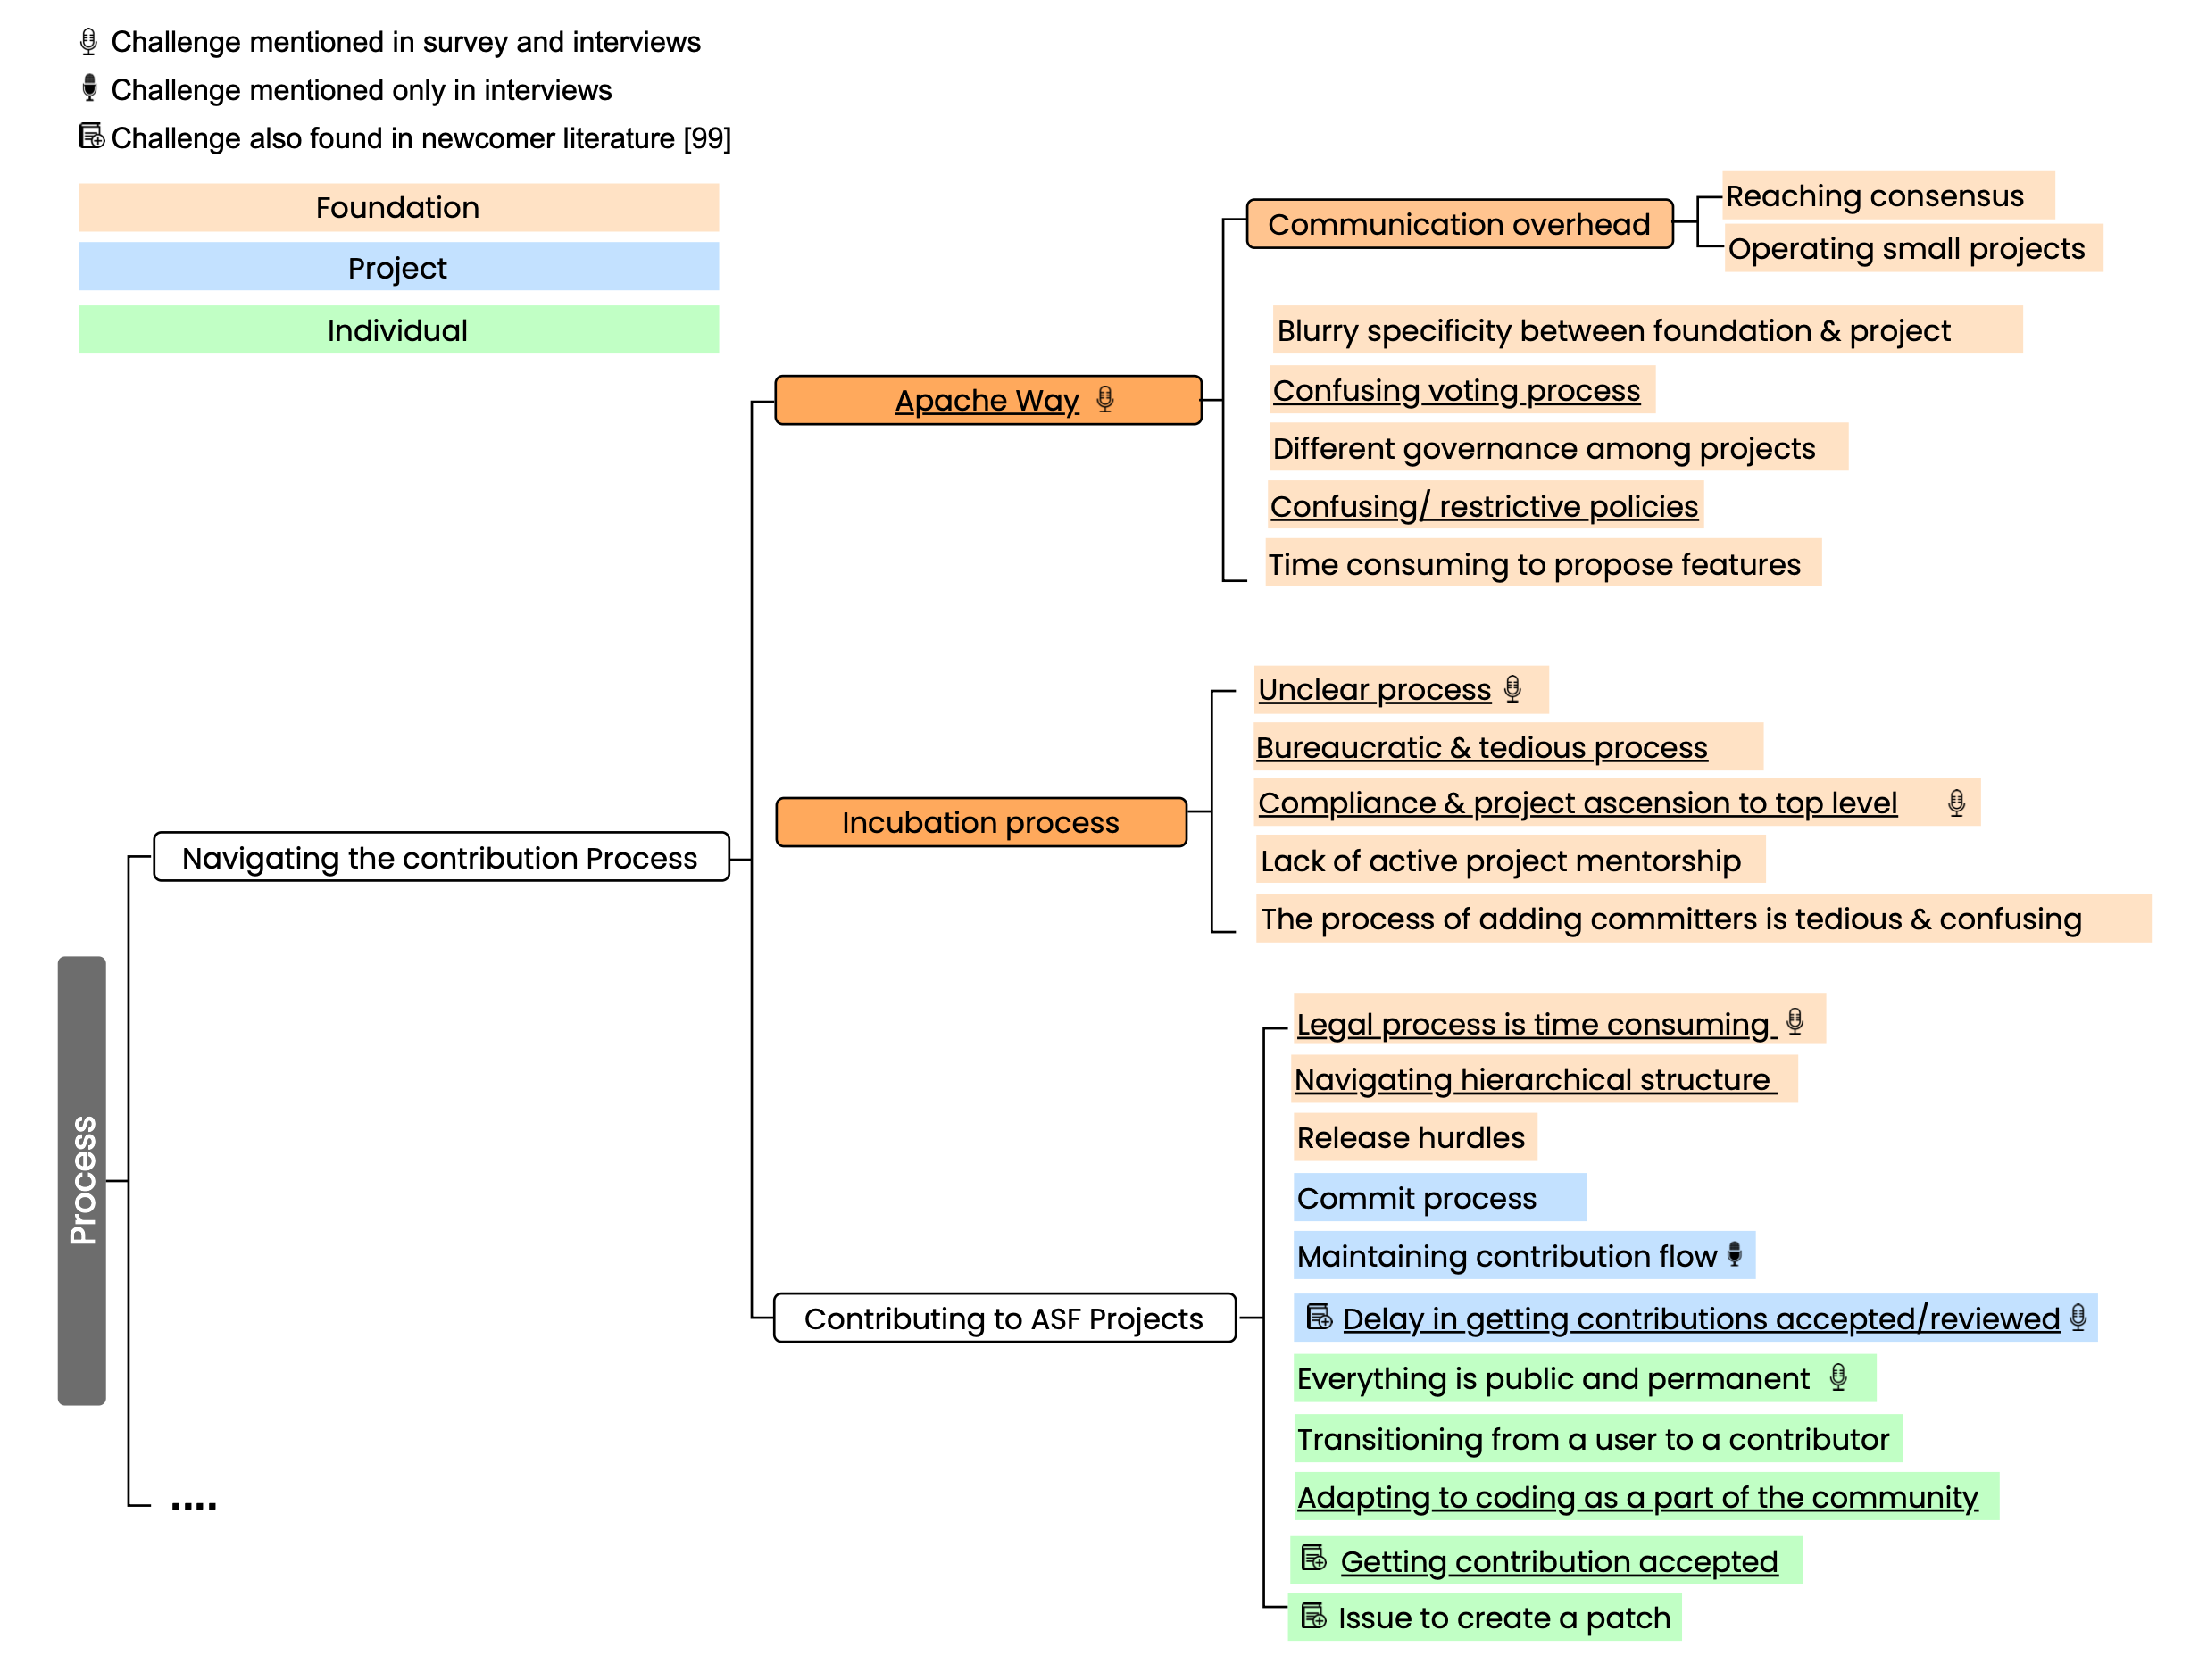
\includegraphics[width=1\linewidth]{figs/processChallenges.png}
    \caption{Challenges faced by developers contributing to ASF projects \citep{04guizani2021long}}
    \label{fig:processChallenges}
\end{figure}


In corporate settings, product development teams often adhere to a rigid process, like Agile or Scrum, with clear roles, responsibilities, and hierarchies. Conversely, open-source projects operate more flexibly, with contributors often taking on diverse roles. This lack of formal structure can be challenging for newcomers, who may find it difficult to identify decision-makers, understand governance, or navigate informal power dynamics within the community.


Adherence to coding standards and contribution guidelines is another significant hurdle. Each project has its own meticulously crafted conventions and best practices, often accumulated over years of development. Failing to comply with these standards can lead to rejected contributions or frustrating delays in getting changes merged. For newcomers, who are still acclimating to the project's culture and technical requirements, this can be a discouraging experience.

Compounding these challenges is the frequent lack of comprehensive and user-friendly onboarding materials. While some projects may boast extensive documentation, it is often not tailored for newcomers or may be outdated, leaving crucial information buried or irrelevant. The absence of step-by-step tutorials that walk newcomers through the contribution process, clear explanations of the project's architecture and codebase, or readily available mentorship programs can leave them feeling lost and overwhelmed. This lack of guidance not only discourages potential contributors but also hinders their ability to make meaningful contributions, ultimately depriving the project of valuable talent and fresh perspectives.

Moreover, developers may find certain open-source projects terrifying due to their immense scale and intricacy. With vast codebases, numerous contributors, and a long history of development, it can be difficult to know where to start or how to make a meaningful impact. The lack of a structured onboarding process, coupled with the fear of making mistakes or not understanding the project's intricacies, can create a sense of paralysis and prevent newcomers from taking that crucial first step.



\clearpage